
\section{Evaluation}
\label{eval}
In this section, we discuss our experimental results. We run experiments in 2-, 4-, and 8-node clusters to measure the scale out feature of the systems under test. Throughout the experiments we used Storm 1.0.2, Spark 2.0.1 and Flink 1.1.3.  The experiments are done with the maximum and 90\% sustainable throughputs. Throughout the experiments, each DI generates 100M events and we use 16 parallel DIs in the cluster. 
%\todo[inline]{Why does a DI have an *input* size? Do you mean the total number of records generated?->fixed} 
We allocate 16 CPUs and 16GB RAM for every node. %\todo[inline]{what does this mean? what does a server have per node? and what engine do you mean?=>fixed} 
All nodes' system clocks in the cluster are synchronized via an NTP server. We generate events with normal distribution.\todo[inline]{what does it mean normla distribution here? With respect to which field?} The network bandwidth is 1Gb/s. We only use processing time windows in the experiments as it is the only window type that all three systems support. We conducted experiments with event time windows with Storm and Flink; however, the results were very similar to the experiments with processing time windows; therefore, we provide only latter in this paper. 
%\todo[inline]{actually, maybe it would be interesting to add event time windows for Storm and Flink=>currently we cannot do it, because of time limitation}. 
We select $q^{a}$ to be 5\% and $q^{b}$ 10 \% of the overall input. Although we did experiments with lower values of the particular variables, it was hard to detect the systems' maximum sustainable throughput. The reason is that  the systems under test use pull-based mechanism to get data from DQS and and the smaller the queue size the more difficult to test SUT's upper limit workload.  We use approximately 25\% of the input data as a warmup. So, in all experiments we exclude the first 25\% of output. The backpressure is enabled in all systems to ensure the durability of experiments. That is, we do not want the systems to ingest more input than they can process and crash during the experiment. In preliminary experiments, measuring the maximum throughput without backpressure mechanisms lead to various exceptions. If the SUT drops one or more connections to the DI, then the experiment is halted with the conclusion that the SUT cannot sustain the given throughput. Similarly, in real-life if the system cannot sustain the user feed and drops connection, then this is considered as a failure.  

\textbf{Tuning the systems.}
Tuning the engines' configuration parameters is important to get a good performance for the given use-cases. %\todo[inline]{what are aggregation partitioned windows?=>fixed}
There are several properties for each SDPS, that need to be tuned to customize the given use-case. For example, in Flink the buffer size has to be adjusted properly to ensure a good balance between throughput and latency. Although selecting low buffer sizes can result in low system latency, the actual latency of tuples may increase as they will be queued in the DQI instead of the buffers inside the system. In Spark the block interval for partitioning the RDDs is one key aspect to tune the system for the given use-case. The number of RDD partitions a single mini-batch  is bounded by $batchInterval \ / \ blockInterval$. As the cluster size increases, decreasing the block interval can increase the parallelism. One of the main reasons that Spark scales up very well is the partitioning of RDDs. However, depending on the use-case, the optimal number of RDD partitions can change. In Storm the number of workers, executors and buffer size are the the configurations (among many other) that needs to be tuned to get the best performance. Similar to Flink, choosing the buffer size is a key to balance between latency and throughput. For all systems,  choosing the right parallelism level is essential to balance between a good resource utilization and network or resource exhaustion.
%\todo[inline]{can you comment on the parameters that you set and how you determined the right parameters? This would be more helpful then just saying that this needs to be done=>below}




\textbf{Windowed operations.} \textcolor{red}{When talking about the windowed queries, we should take the system architecture into the consideration. For example, Spark gathers the data in window and then parallelizes the computation within a single window. Basically, it enables users to query a single window. We call it global windows. Flink and Storm on the other hand, first partitions the data and then creates windows. As a result, user queries much smaller(depending on data skew) partitioned windows. However, there is no coordination between partitioned windows. As a result, there is no guarantee that one set of windows will be processed after another. We call this approach partitioned windows. 
	In all previous works, this difference was neglected. Spark supports only global windows but Flink and Storm supports both types. Throughout our evaluations, we evaluate both cases for Flink and Storm and compare with Spark.  }

\textbf{Partitioned Windowed Aggregations.}
In the first use-case, we use parti\-tioned  windowed aggregations in Storm, Spark, and Flink. We calculate the maximum sustainable  throughput for  each SDPS. To confirm that the engines are saturated, we performed the same experiments with 90\% of the maximum throughput. We calculate the latency measurements for each system over the respective throughputs.  

    \begin{table*}
        \resizebox{\textwidth}{!} {\begin{tabular}{lllll}\toprule
            &\textbf{2-node}  & \textbf{4-node} & \textbf{8-node}\\\midrule
            Storm & 1407, 66, 5758, (2330, 2721, 3477) & 2058, 115, 12216, (3724, 5856, 7767) & 2253, 179, 17762, (3818, 6467, 9245) \\
            Storm(90\%) & 1100, 84, 5752, (1832, 2176, 2859) & 1676, 43, 9280, (2985, 4140, 6330) & 1932, 182, 11040, (3324, 5005, 7630) \\
            Spark & 3673, 2537, 8596, (4603, 4953, 5990) & 3394, 1987, 6994, (4076, 4315, 4955) & 3139, 1223, 6946, (3896, 4162, 4711)\\
            Spark(90\%) & 3416, 2354, 8005, (3936, 4550, 5443) & 2822, 1630, 6925, (3473, 3767, 4804) & 2781, 1702, 5961, (3624, 3948, 4834)\\
            Flink & 563, 4, 12328, (1448, 2282, 5233) & 265, 4, 5132, (612, 1242, 2479) & 258, 4, 5469, (574, 1228, 3975) \\
            Flink(90\%) & 310, 3, 5826, (698, 1185, 2009) & 250, 4, 5112, (601, 1334, 2430)  & 219, 2, 5405, (482, 843, 3458) \\
        \end{tabular}}
        \caption{ Latency statistics, avg, min, max, and quantiles (90, 95, 99) in milliseconds for windowed aggregations. \todo[inline]{This should be transformed to an actual table with named columns for the metrics (I know it's difficult but it can be done.)}}
         \label{tab_lat_agg}
    \end{table*} 



    \begin{table}
        \begin{tabular}{lllll}\toprule
            &\textbf{2-node}  & \textbf{4-node} & \textbf{8-node}\\\midrule
            Storm & 408K & 696K & 992K  \\
            Spark & 379K & 642K & 912K  \\
            Flink & 1230K & 1260K & 1260K  \\
        \end{tabular}
        \caption{Sustainable throughput for windowed aggregations. }
        \label{tab_th_agg}
    \end{table} 


%\usepgfplotslibrary{statistics}
\pgfplotsset{compat=1.8}
\usetikzlibrary{pgfplots.statistics}
\makeatletter
\newcommand*\bigcdot{\mathpalette\bigcdot@{1.2}}
\newcommand*\bigcdot@[2]{\mathbin{\vcenter{\hbox{\scalebox{#2}{$\m@th#1\bullet$}}}}}
\makeatother


\makeatletter
\newenvironment{customlegend}[1][]{%
    \begingroup
    % inits/clears the lists (which might be populated from previous
    % axes):
    \pgfplots@init@cleared@structures
    \pgfplotsset{#1}%
}{%
    % draws the legend:
    \pgfplots@createlegend
    \endgroup
}%

% makes \addlegendimage available (typically only available within an
% axis environment):
\def\addlegendimage{\pgfplots@addlegendimage}
\makeatother



\begin{figure}

\begin{tikzpicture}

\begin{axis}[
scaled y ticks = false,
legend entries={simulation,
                measurement,
                sample 1}, 
                legend style={at={(axis cs:6.0,0.84)},anchor=south west},
boxplot/draw direction=y,
ylabel={Latency (millisecond)},
height=4cm,
boxplot={
    %
    % Idea: 
    %  place the 
    %  group 1 at 0.3333 and 0.6666
    %  group 2 at 1.3333 and 1.6666
    %  group 3 at 2.3333 and 2.6666
    %  ...
    % in a formular:
    draw position={1/4 + floor(\plotnumofactualtype/3) + 1/5*mod(\plotnumofactualtype,3)},
    %
    % that means the box extend must be at most 0.33333 :
    box extend=0.1,
},
% ... it also means that 1 unit in x controls the width:
x=1cm,
% ... and it means that we should describe intervals:
xtick={0,1,2,...,10},
ytick={0, 500,10000},
x tick label as interval,
xticklabels={%
    {\tiny 2-node \\ max th.},%
    {\tiny 2-node \\ 90 \% th.},%
    {\tiny 4-node \\ max th.},%
    {\tiny 4-node \\ 90 \% th.},%
    {\tiny 8-node \\ max th.},%
    {\tiny 8-node \\ 90 \% th.},%
},
    x tick label style={
        text width=4.5cm,
        align=center
    },
]
\addlegendimage{line legend,green}
\addlegendentry{ \textcolor{red}{\scriptsize{Storm}   }  }
\addlegendimage{line legend,blue}
\addlegendentry{\textcolor{blue}{\scriptsize{Spark}}}
\addlegendimage{line legend,blue}
\addlegendentry{\textcolor{black}{\scriptsize{Flink}}}
    % 2 node 100
\addplot[color=red,
    boxplot prepared={
      average=1407,
      lower whisker=66,
      upper whisker=5758,
      lower quartile=168,
      upper quartile=3477,
      median=1100
    },
    ] coordinates {};
    
\addplot[color=blue,
    boxplot prepared={
      average=3673,
      lower whisker=2537,
      upper whisker=8596,
      lower quartile=340,
      upper quartile=5990,
      median=2578
    },
    ] coordinates {};
    
    
\addplot[color=black,
    boxplot prepared={
      average=563,
      lower whisker=4,
      upper whisker=12328,
      lower quartile=15,
      upper quartile=5233,
      median=161
    },
    ] coordinates {};
    % 2 node 90
\addplot[color=red,
    boxplot prepared={
      median=1,
      upper quartile=1.2,
      lower quartile=0.4,
      upper whisker=1.5,
      lower whisker=0.2
    },
    ] coordinates {};
    
    
\addplot[color=blue,
    boxplot prepared={
      median=1,
      upper quartile=1.2,
      lower quartile=0.4,
      upper whisker=1.5,
      lower whisker=0.2
    },
    ] coordinates {};
\addplot[color=black,
    boxplot prepared={
      median=1,
      upper quartile=1.2,
      lower quartile=0.4,
      upper whisker=1.5,
      lower whisker=0.2
    },
    ] coordinates {};
    
        % 4 node 100
    \addplot[color=red,
    boxplot prepared={
      median=1,
      upper quartile=1.2,
      lower quartile=0.4,
      upper whisker=1.5,
      lower whisker=0.2
    },
    ] coordinates {};
    
    
\addplot[color=blue,
    boxplot prepared={
      median=1,
      upper quartile=1.2,
      lower quartile=0.4,
      upper whisker=1.5,
      lower whisker=0.2
    },
    ] coordinates {};
\addplot[color=black,
    boxplot prepared={
      median=1,
      upper quartile=1.2,
      lower quartile=0.4,
      upper whisker=1.5,
      lower whisker=0.2
    },
    ] coordinates {};
    
            % 4 node 90
    \addplot[color=red,
    boxplot prepared={
      median=1,
      upper quartile=1.2,
      lower quartile=0.4,
      upper whisker=1.5,
      lower whisker=0.2
    },
    ] coordinates {};
    
    
\addplot[color=blue,
    boxplot prepared={
      median=1,
      upper quartile=1.2,
      lower quartile=0.4,
      upper whisker=1.5,
      lower whisker=0.2
    },
    ] coordinates {};
\addplot[color=black,
    boxplot prepared={
      median=1,
      upper quartile=1.2,
      lower quartile=0.4,
      upper whisker=1.5,
      lower whisker=0.2
    },
    ] coordinates {};

            
            % 8 node 100
\addplot[color=red,
    boxplot prepared={
      median=1,
      upper quartile=1.2,
      lower quartile=0.4,
      upper whisker=1.5,
      lower whisker=0.2
    },
    ] coordinates {};
    
    
\addplot[color=blue,
    boxplot prepared={
      median=1,
      upper quartile=1.2,
      lower quartile=0.4,
      upper whisker=1.5,
      lower whisker=0.2
    },
    ] coordinates {};
\addplot[color=black,
    boxplot prepared={
      median=1,
      upper quartile=1.2,
      lower quartile=0.4,
      upper whisker=1.5,
      lower whisker=0.2
    },
    ] coordinates {};

            
            
             % 8 node 90
 \addplot[color=red,
    boxplot prepared={
      median=1,
      upper quartile=1.2,
      lower quartile=0.4,
      upper whisker=1.5,
      lower whisker=0.2,
       average = 4.05
    },
    ] coordinates {};
    
    
\addplot[color=blue,
    boxplot prepared={
      median=1,
      upper quartile=1.2,
      lower quartile=0.4,
      upper whisker=1.5,
      lower whisker=0.2
    },
    ] coordinates {};
\addplot[color=black,
    boxplot prepared={
      median=1,
      upper quartile=1.2,
      lower quartile=0.4,
      upper whisker=1.5,
      lower whisker=0.2
    },
    ] coordinates {};


\end{axis}

\end{tikzpicture}
\caption{dede}
\end{figure}


The maximum sustainable throughput of the SDPSs are shown in Table \ref{tab_th_agg}. We use a four second batch-size for  Spark, as it can sustain the  maximum throughput with this configuration. We identified that for 4- and 8-node configurations, Flink's performance is bounded by network bandwidth.  Storm's and Spark's performance in terms of throughput are comparable, with Storm outperforming Spark by approximately 8\% in all configurations. One reason for Spark's worse performance can be the  overhead of starting periodic  mini-batch jobs. %\todo[inline]{do not understand->fixed}
Storm and Flink, on the other hand, are operating on tuples and, therefore, can sustain higher sustainable throughputs. % \todo[inline]{That is unintuitive, generally, batch systems have higher throughput but also higher latency->changed throughputs to sustainable throughputs}
 We want to stress that the sustainable throughput is not the same as an engine's peak throughput. %  \todo[inline]{Why is the mini batch architecture reason for that?=>deleted}
 As stated above, we are interested in measuring maximum sustainable  throughputs of SUTs in this paper.  We adjusted Spark's block interval to achieve a better parallelism on RDD level and the highest sustainable throughput. Storm introduced  backpressure feature in recent releases; however, it is not mature yet. With high workloads, it is possible that the backpressure stalls the topology, causing spouts to stop emitting tuples. Moreover, we notice that Storm  drops some connections to the DIs when tested with high workloads with backpressure disabled, which is not acceptable according to the real world use-cases. Dropping connections due to high throughput is considered  a system failure.


Table \ref{tab_lat_agg} shows the latency measurements of windowed aggregations. We conduct experiments with the maximum and 90\%-workloads and report $avg$, $min$, $max$, and  quantiles (90,95,99) over the results. %\todo[inline]{fix quantiles->fixed} 
 The latencies shown in this table are computed with the workloads given in Table \ref{tab_th_agg}.  In most cases, where the network bandwidth is not a bottleneck, we can see a significant decrease in latency when lowering the throughput by 10\%. This shows that the maximum throughput saturates the system.  For example, Flink's metrics shown in Table  \ref{tab_lat_agg} change more than the metrics of other systems when lowering the throughput. The reason is that it pulls the data from DQS more periodically than other systems so that the queue size does not get beyond the limits. 
 Spark's 2-node configuration, on the other hand, exhibits negligible difference in latency measurements between the maximum and 90\% sustainable throughputs.  The reason is that for that configuration, Spark cannot pull the data from DQS periodically and therefore the queue size goes beyond accepted limits. As a result, we do the benchmarks with lower throughputs. 
This also shows the efficiency of backpressure feature in systems under test. The smoother the backpressure and the lower the overhead of backpressure, the easier to saturate the system with sustainable throughput. 

Flink has the best $min$ and $avg$ latencies. Although its $max$ latency is way above its $min$, from quantile values we can conclude that those values can be considered as outliers. The main reason for having such a high $max$ latency is associated with the buffer size. The large buffer size enables high throughput; on the other hand, it can cause some tuples to have high latencies. For example, with a larger buffer size the tuple resides in buffer longer until the buffer gets filled and flushes. In the 4- and 8-node cluster configurations, we can see that there is a slight difference in Flink's latency statistics between  the maximum and 90\%-throughputs. The reason is that this workload is not the maximum sustainable throughput but is bounded by the network bandwidth. %\todo[inline]{Maybe add a note on the total network transfer / throughput based on the tuple size and throughput - I ADDED NETWORK/CPU UTILIZATION FIGURES. SHOULD THEY BE ENOUGH FOR THIS ISSUE?}
 
As we see from Table \ref{tab_lat_agg},  Spark has more latency than Storm and Flink but it exhibits less of a difference among the $avg$, $min$, and $max$ latency measurements. Because it processes tuples in mini-batches, the tuples within the same batch have similar latencies; therefore, there is no huge difference among measurements. Moreover, transferring the data from Spark's block manager to DStream by creating RDDs is another overhead that results in Spark's higher $avg$ latency compared to Flink and Storm.  Although the $avg$ and $max$ latencies increase in Storm with increasing workload and cluster size, in Spark we see the opposite behavior, which means Spark can partition the data (RDDs) in bigger distributed environments. However, from the quantile values we can conclude that the $max$ latencies of Storm  can be considered as outliers.








\textbf{Global Windowed Aggregations.}
\textcolor{red}{As we discussed above, in global windowed aggregations the system collects the data and parallelizes the query for the data inside window. As a result, the system should be able to manage and parallelize large size windows. Because Spark only supports global windowed aggregations, we enable the global window aggregation semantics in Flink and Storm and compare with Spark. In Flink and Storm, for all types of windowed queries, the performance of the system is bounded by the performance of a single slot of a machine, meaning it does not scale. The reason lies under the design option of a system. That is, supporting querying querying big windows and coordinating the sub-queries of a given query is costly. For Query- 1, we measured the throughput 480K for Flink and 200K for Storm. We can see that on 2 nodes Flink's single threaded global windowed aggregation beats over Spark and Storm. However, Spark imrpoves the performance as it scales as we can see from Table \ref{tab_th_agg}.}































\begin{figure*}
    \centering
    \begin{subfigure}[b]{0.3\textwidth}
        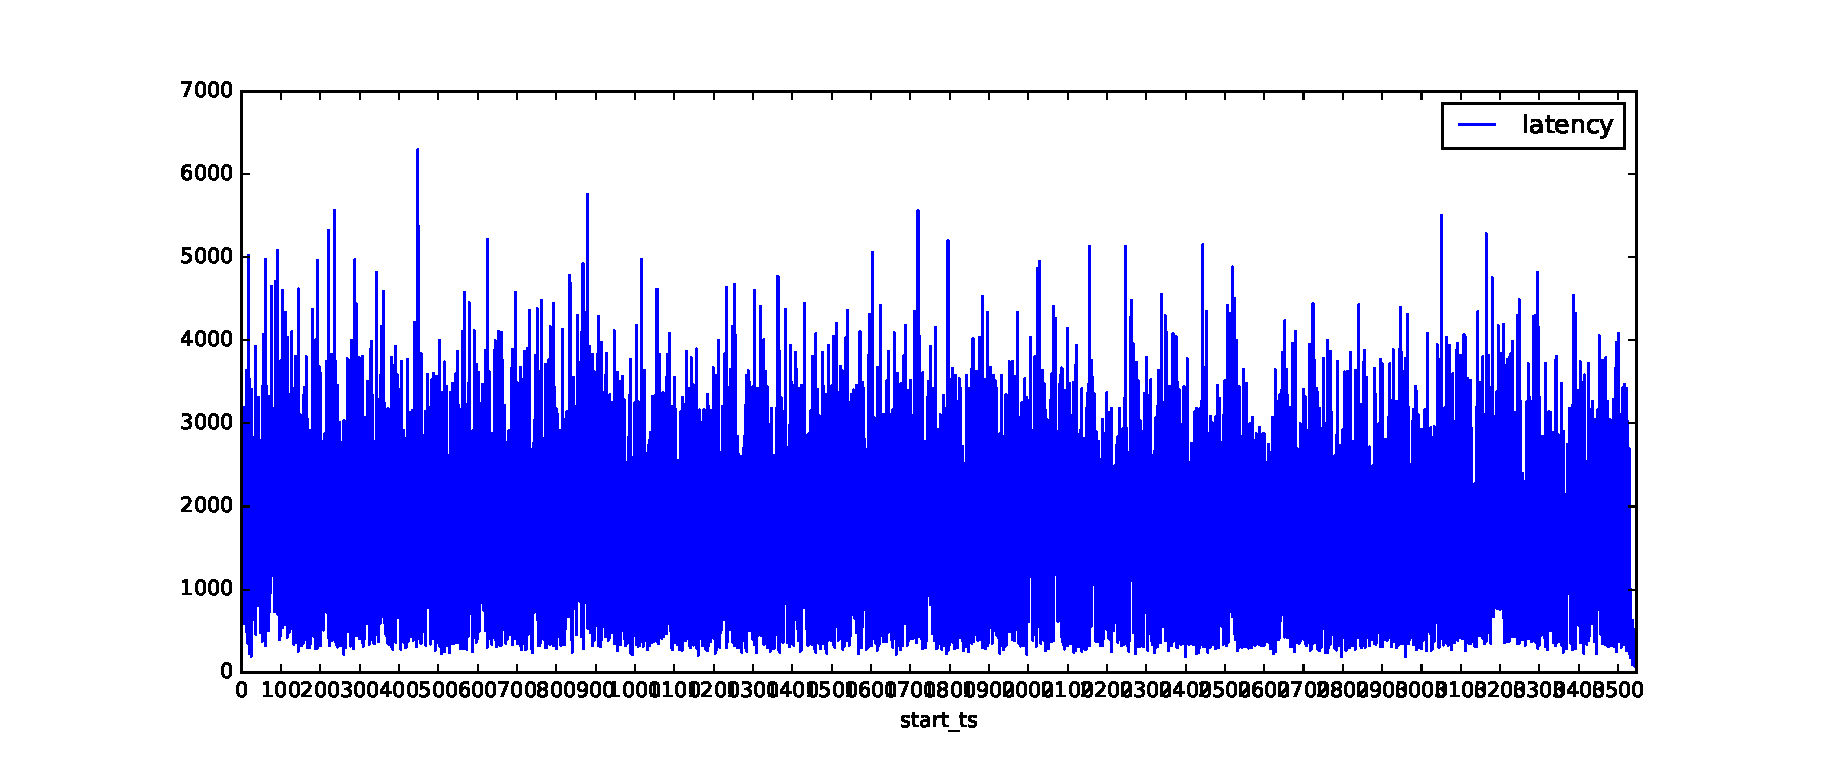
\includegraphics[width=\textwidth]{eps/storm_agg_2node_th_max_ts}

        \caption{Storm, 2-node, max   throughput }
    \end{subfigure}
    ~ 
    \begin{subfigure}[b]{0.3\textwidth}
        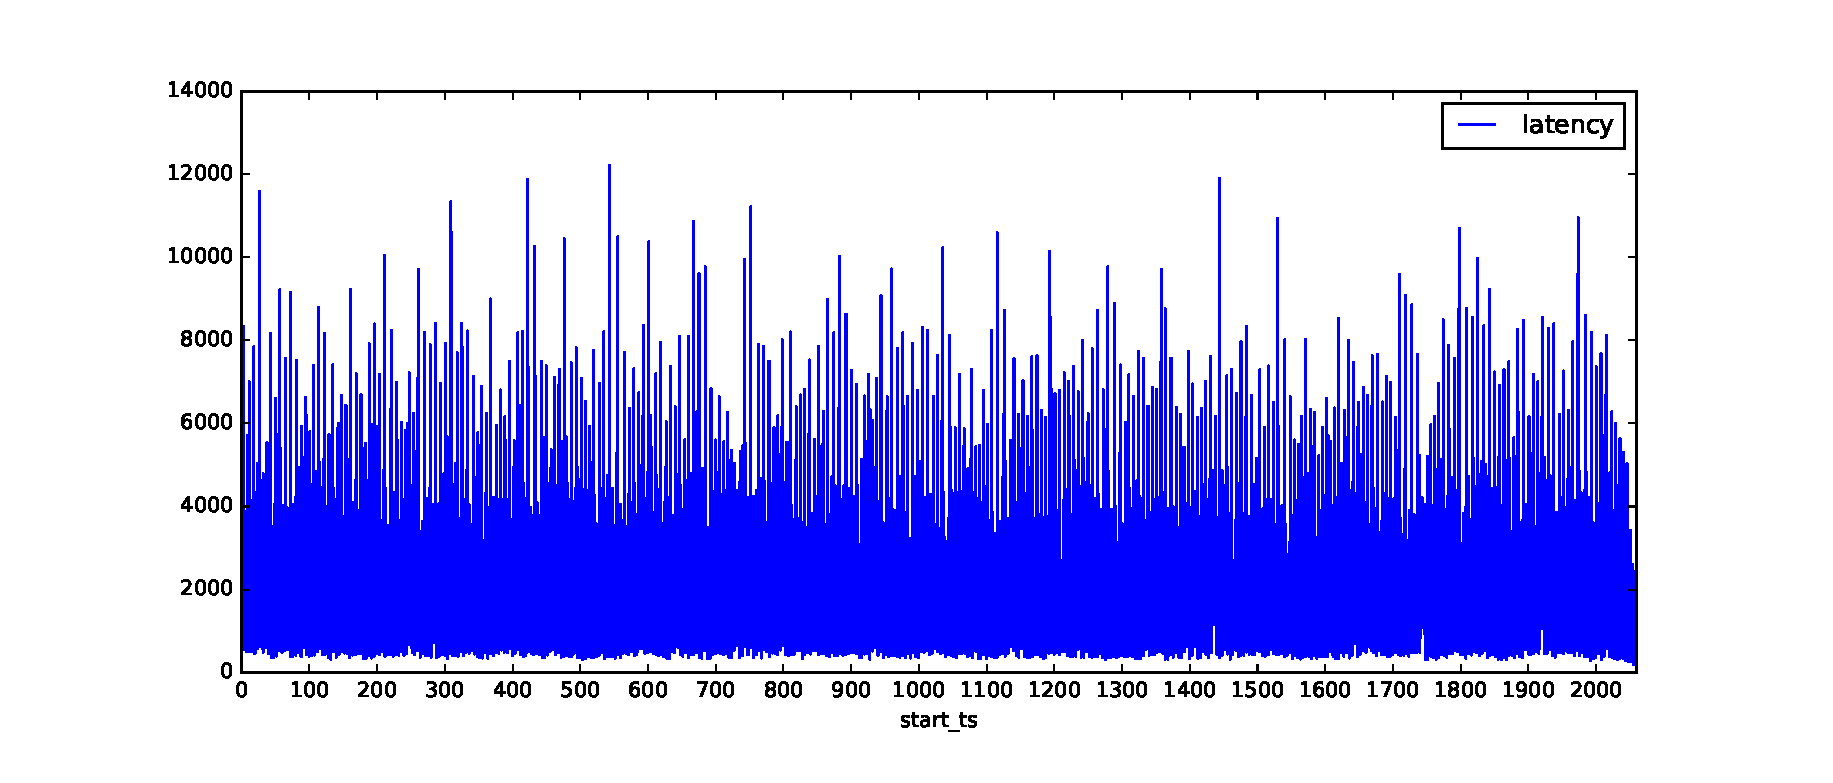
\includegraphics[width=\textwidth]{eps/storm_agg_4node_th_max_ts}

        \caption{Storm, 4-node, max   throughput }
    \end{subfigure}
    ~ 
    \begin{subfigure}[b]{0.3\textwidth}
        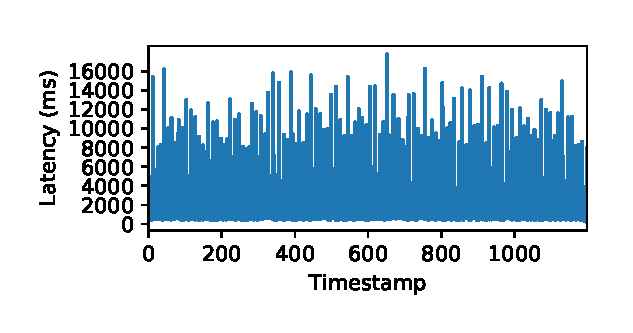
\includegraphics[width=\textwidth]{eps/storm_agg_8node_th_max_ts}

        \caption{Storm, 8-node, max   throughput }
                 \label{fig_storm_agg_8node_th_max_ts}
    \end{subfigure}



    \begin{subfigure}[b]{0.3\textwidth}
        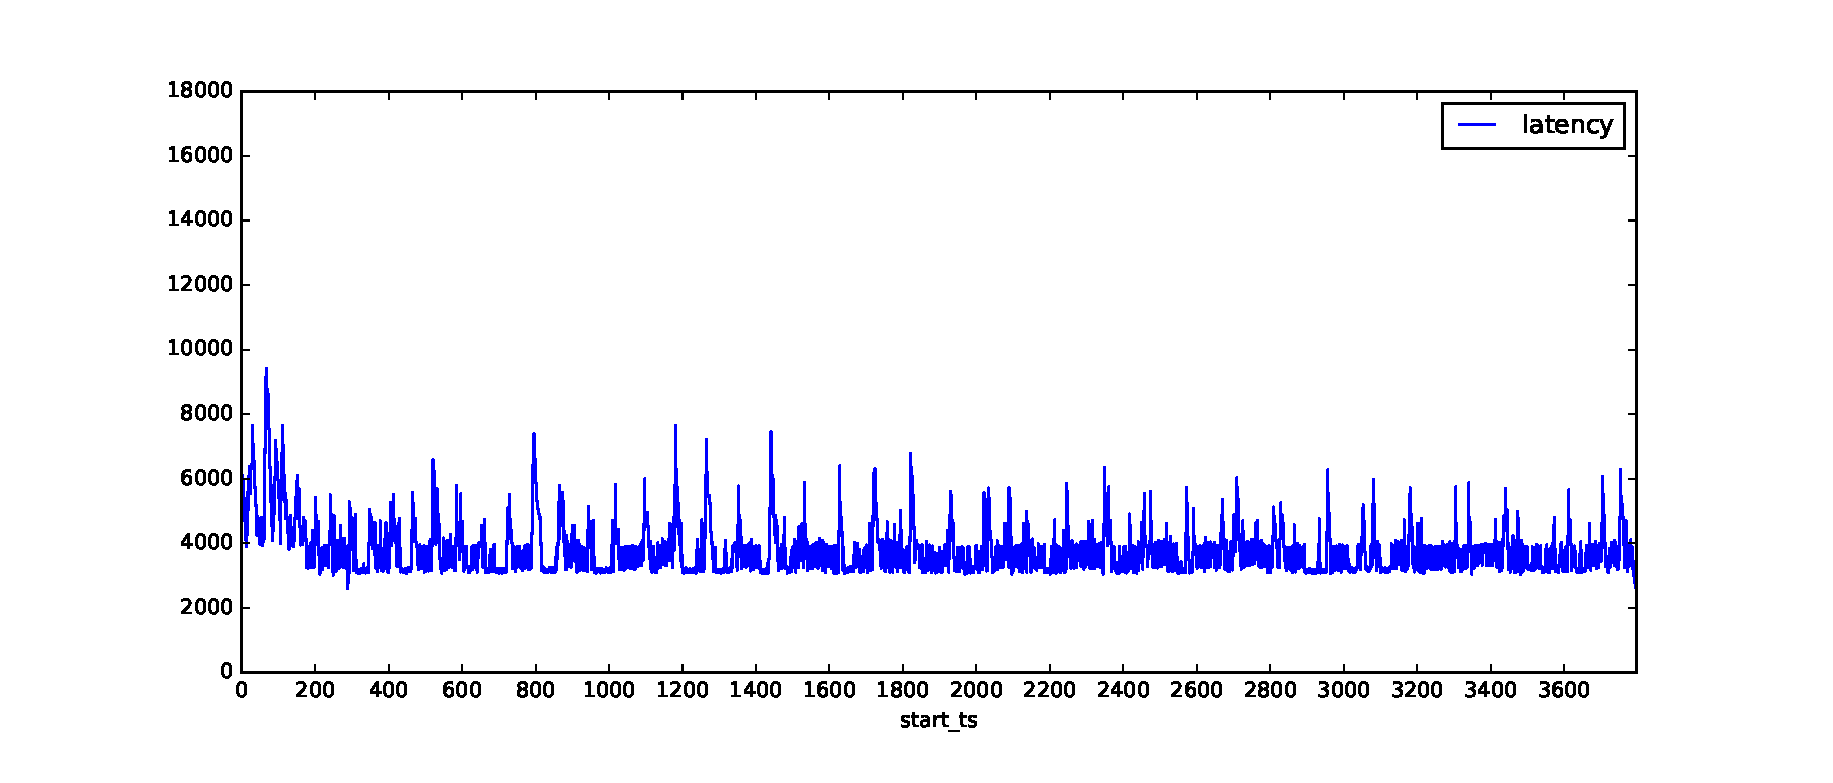
\includegraphics[width=\textwidth]{eps/spark_agg_2node_th_max_ts}

        \caption{Spark, 2-node, max   throughput }
    \end{subfigure}
    ~ 
    \begin{subfigure}[b]{0.3\textwidth}
        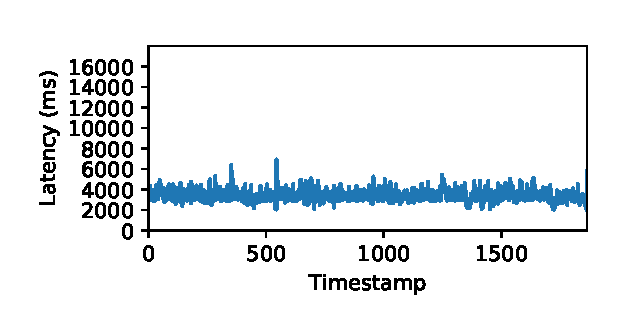
\includegraphics[width=\textwidth]{eps/spark_agg_4node_th_max_ts}

        \caption{Spark, 4-node, max   throughput }
    \end{subfigure}
    ~ 
    \begin{subfigure}[b]{0.3\textwidth}
        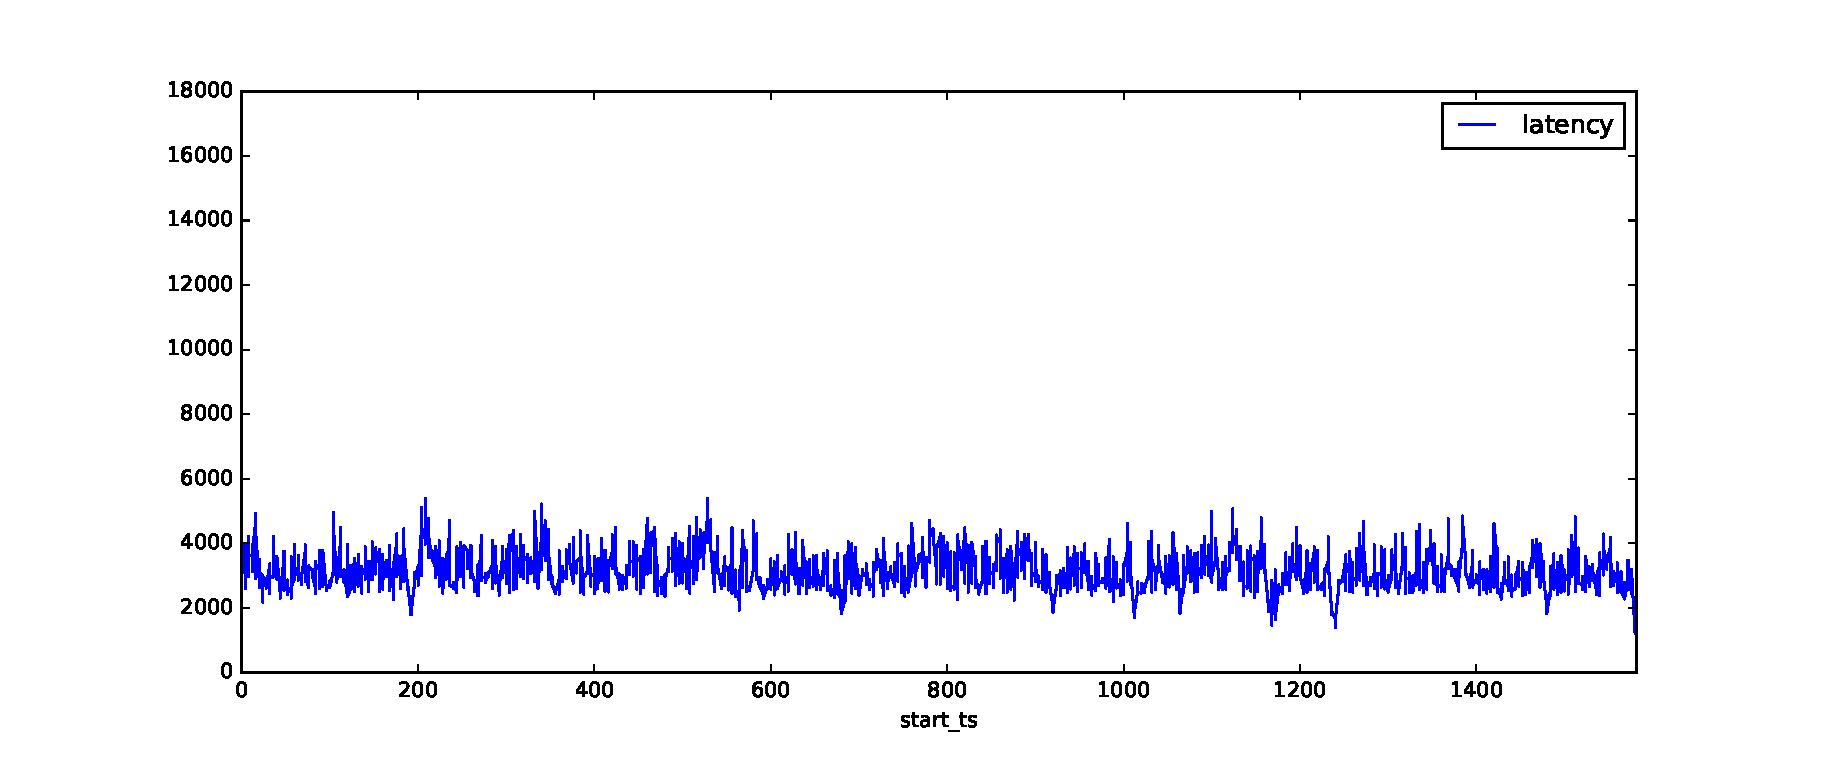
\includegraphics[width=\textwidth]{eps/spark_agg_8node_th_max_ts}

        \caption{Spark, 8-node, max   throughput }
         \label{fig_spark_agg_8node_th_max_ts}
    \end{subfigure}



    \begin{subfigure}[b]{0.3\textwidth}
        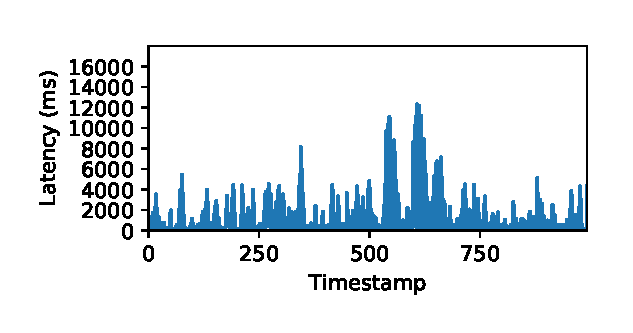
\includegraphics[width=\textwidth]{eps/flink_agg_2node_th_max_ts}

        \caption{Flink, 2-node, max   throughput }
                \label{flink_agg_2node_th_max_ts}

    \end{subfigure}
    ~ 
    \begin{subfigure}[b]{0.3\textwidth}
        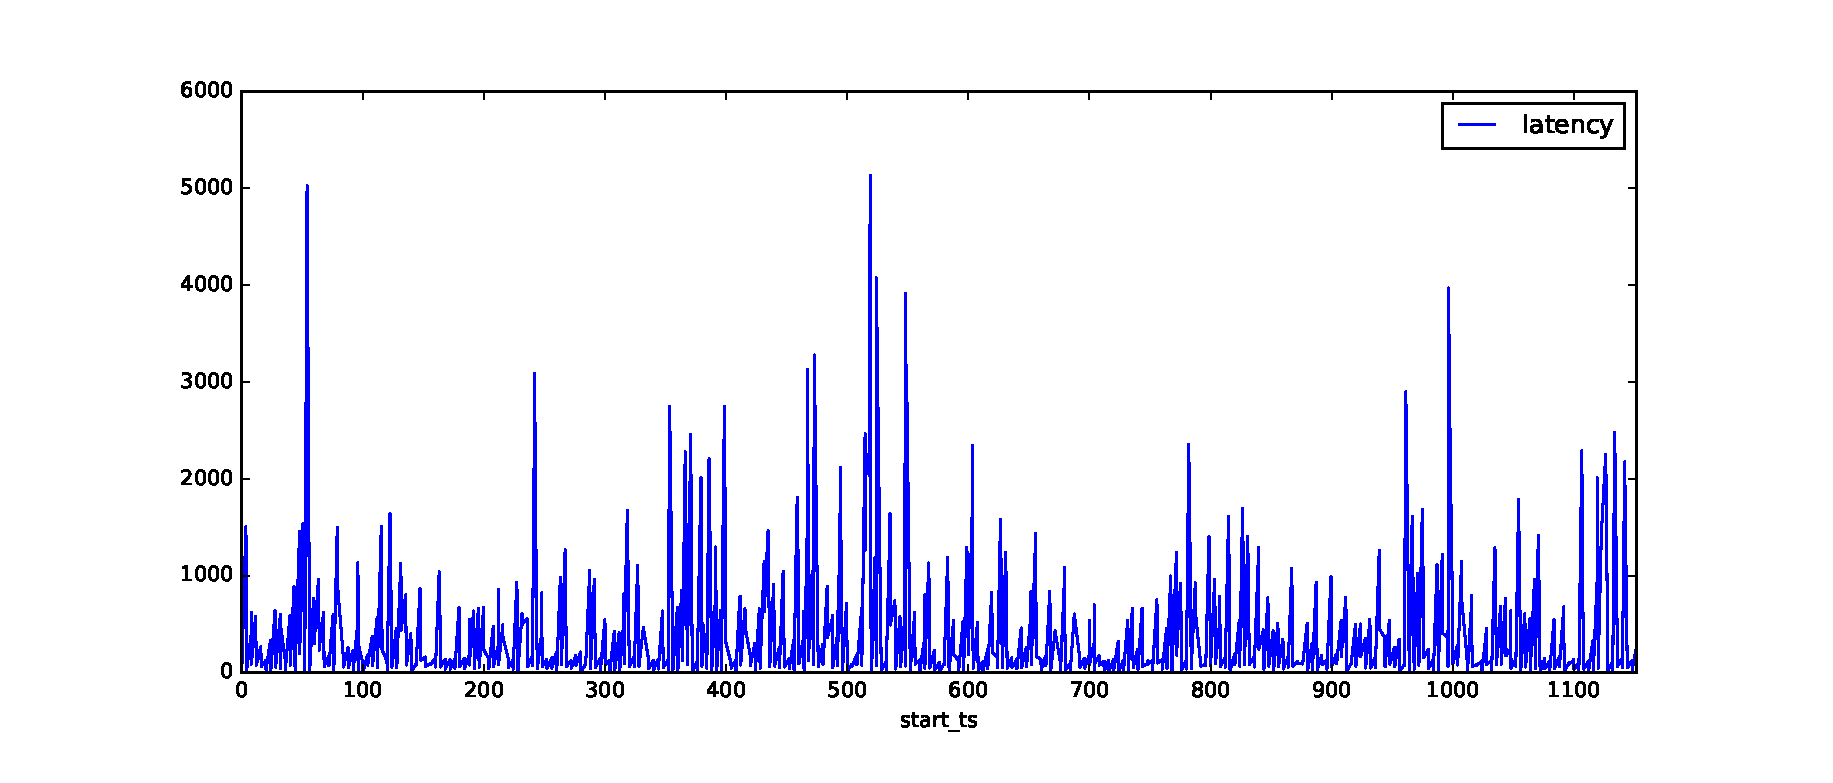
\includegraphics[width=\textwidth]{eps/flink_agg_4node_th_max_ts}

        \caption{Flink, 4-node, max   throughput }
    \end{subfigure}
    ~ 
    \begin{subfigure}[b]{0.3\textwidth}
        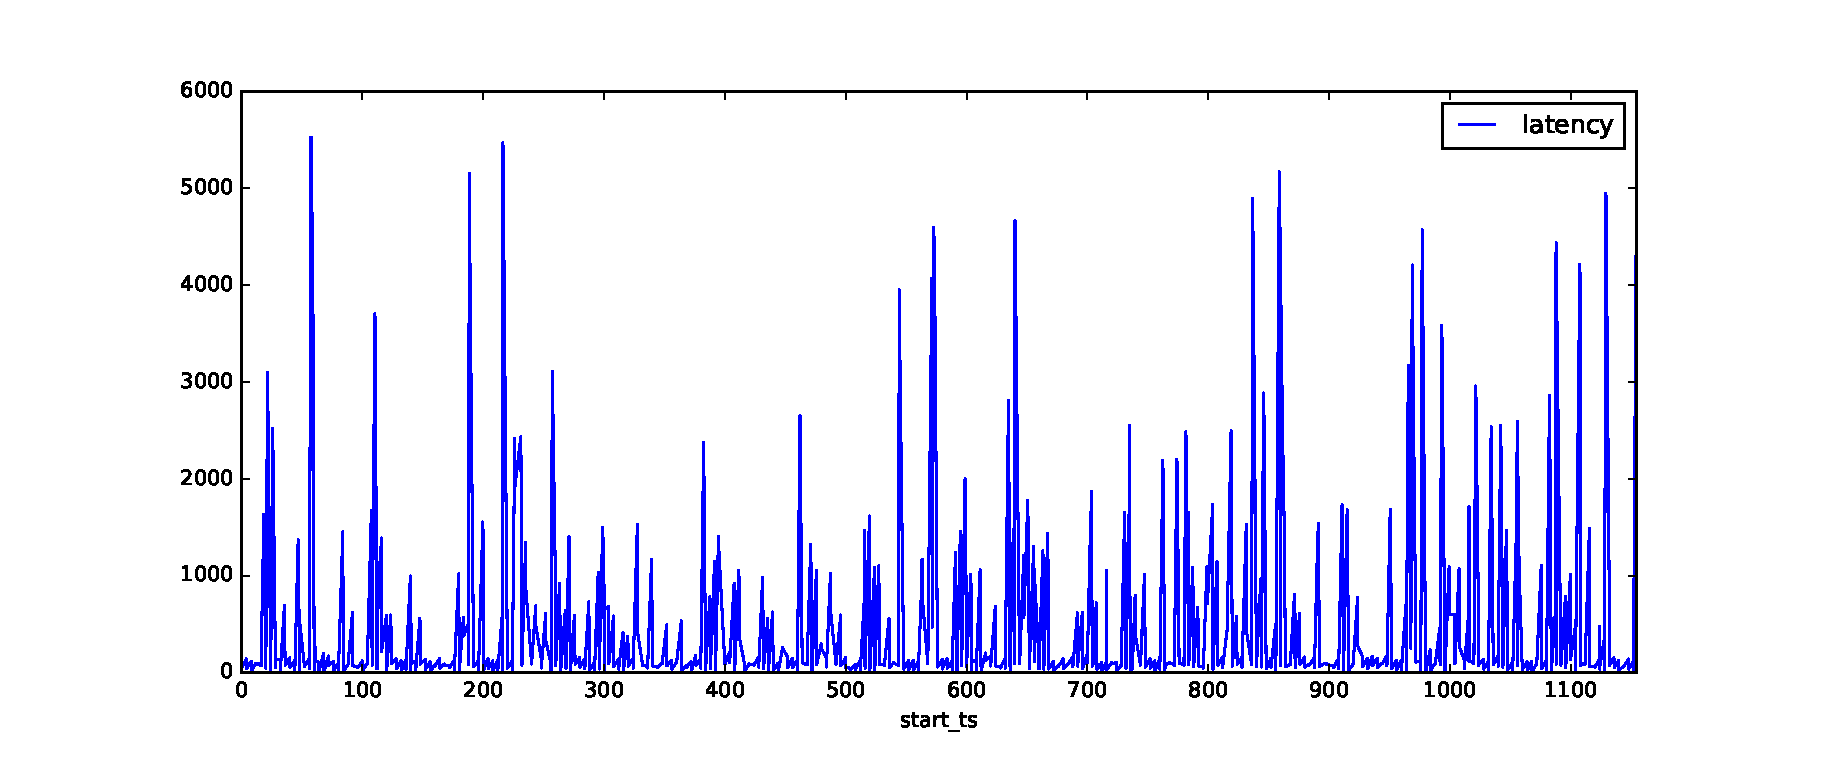
\includegraphics[width=\textwidth]{eps/flink_agg_8node_th_max_ts}

        \caption{Flink, 8-node, max   throughput }
        
    \end{subfigure}




    \begin{subfigure}[b]{0.3\textwidth}
        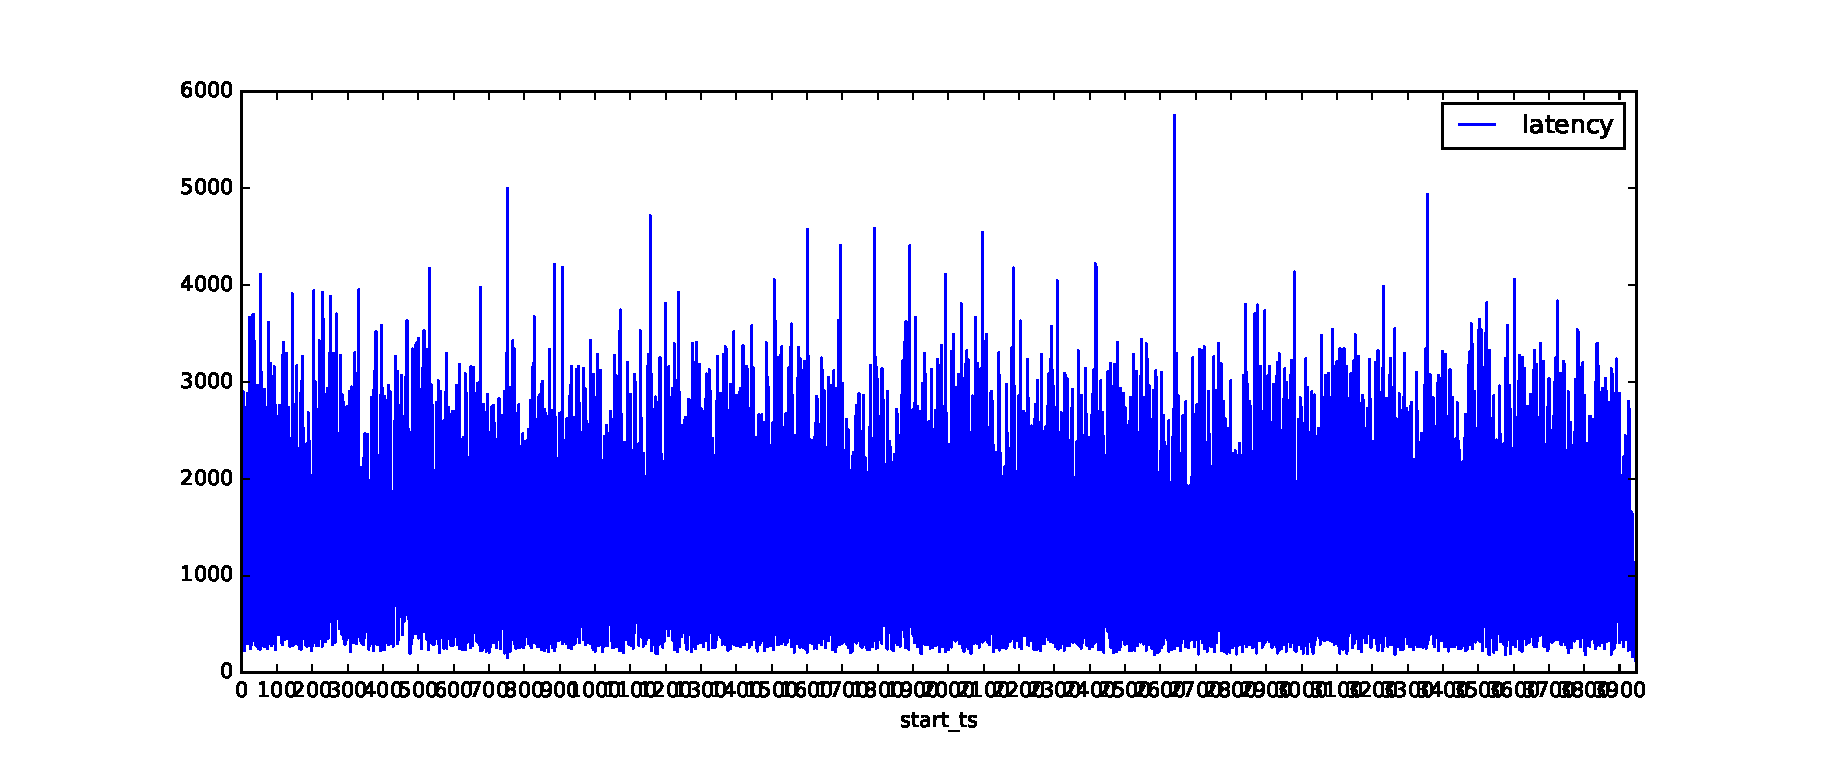
\includegraphics[width=\textwidth]{eps/storm_agg_2node_th_90_ts}

        \caption{Storm, 2-node,  90\%- throughput }
    \end{subfigure}
    ~ 
    \begin{subfigure}[b]{0.3\textwidth}
        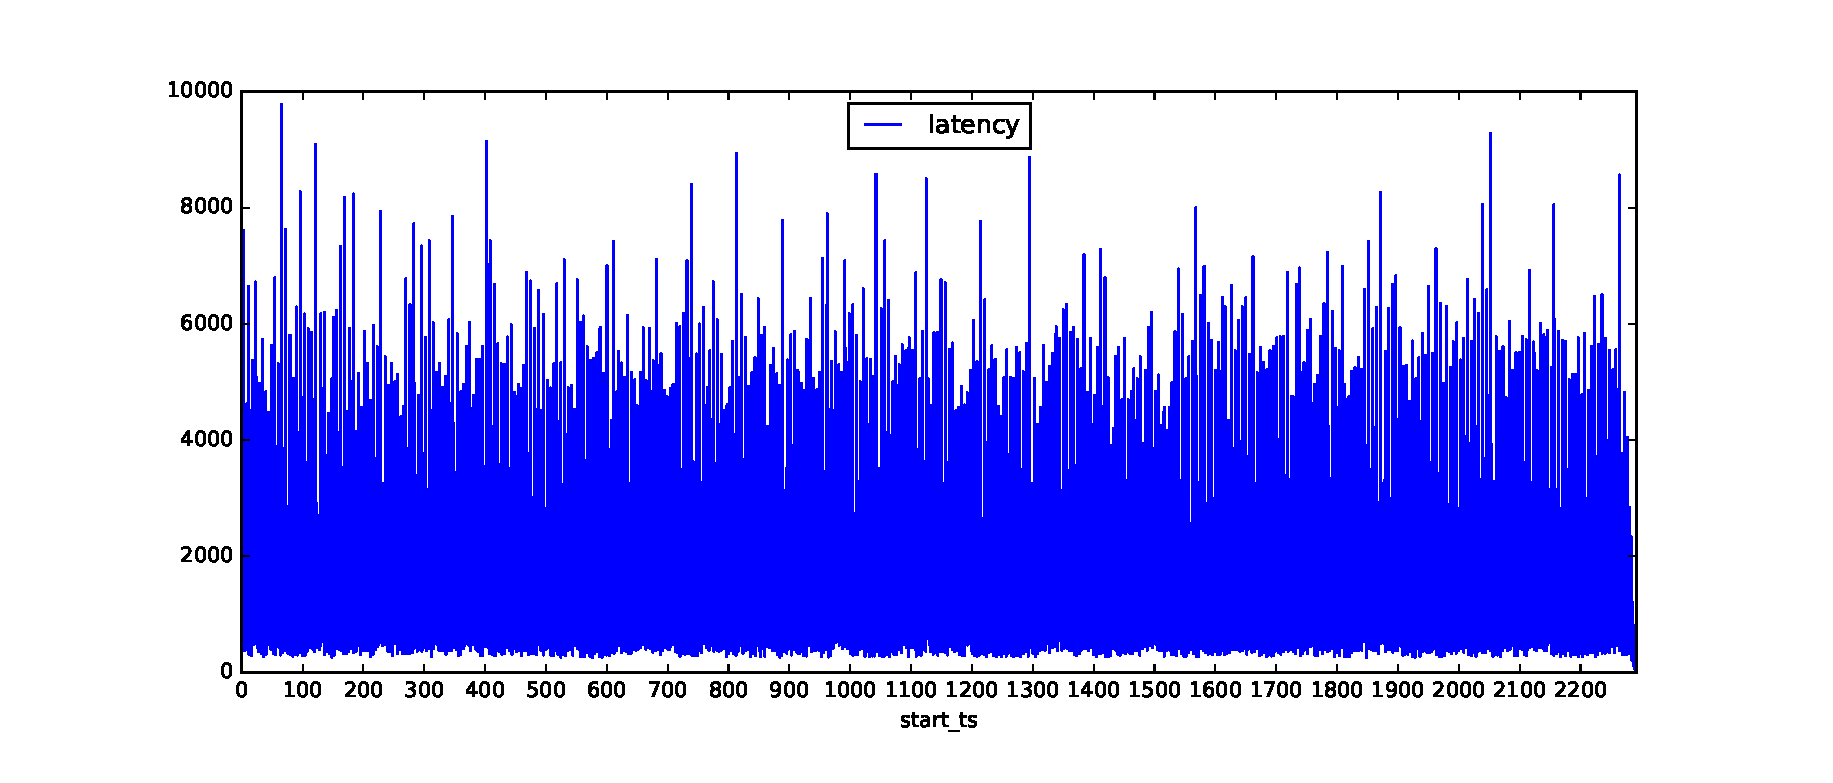
\includegraphics[width=\textwidth]{eps/storm_agg_4node_th_90_ts}

        \caption{Storm, 4-node,  90\%- throughput }
    \end{subfigure}
    ~ 
    \begin{subfigure}[b]{0.3\textwidth}
        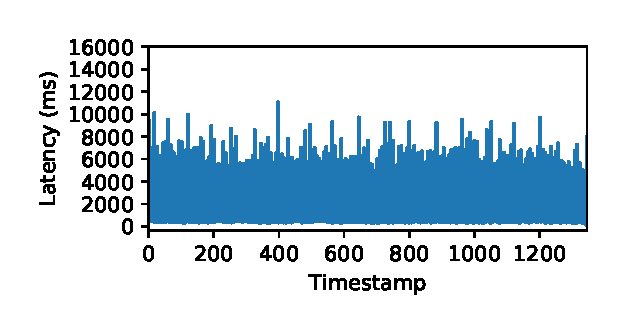
\includegraphics[width=\textwidth]{eps/storm_agg_8node_th_90_ts}

        \caption{Storm, 8-node,  90\%- throughput }
                \label{fig_storm_agg_8node_th_90_ts}
    \end{subfigure}



    \begin{subfigure}[b]{0.3\textwidth}
        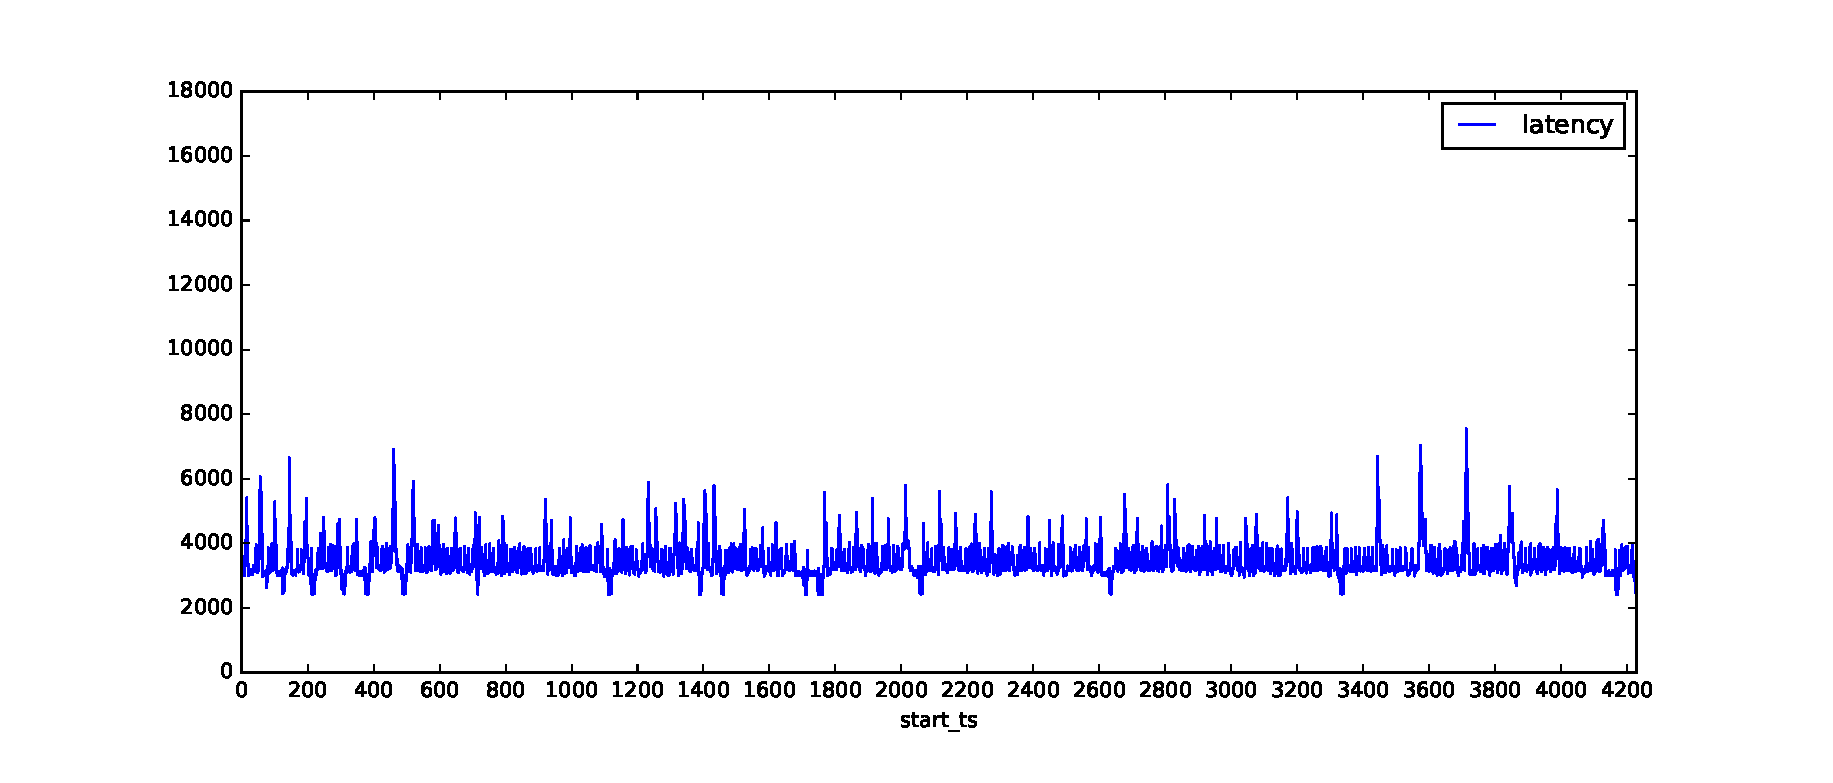
\includegraphics[width=\textwidth]{eps/spark_agg_2node_th_90_ts}

        \caption{Spark, 2-node,  90\%- throughput }
    \end{subfigure}
    ~ 
    \begin{subfigure}[b]{0.3\textwidth}
        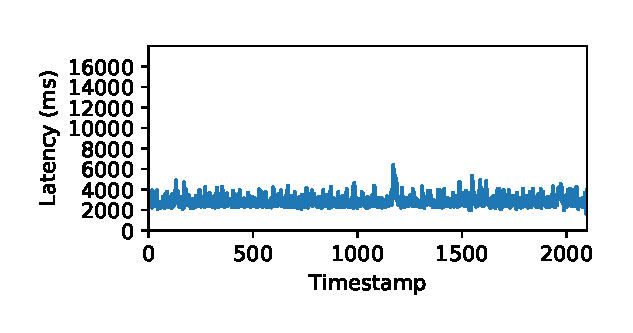
\includegraphics[width=\textwidth]{eps/spark_agg_4node_th_90_ts}

        \caption{Spark, 4-node,  90\%- throughput }
    \end{subfigure}
    ~ 
    \begin{subfigure}[b]{0.3\textwidth}
        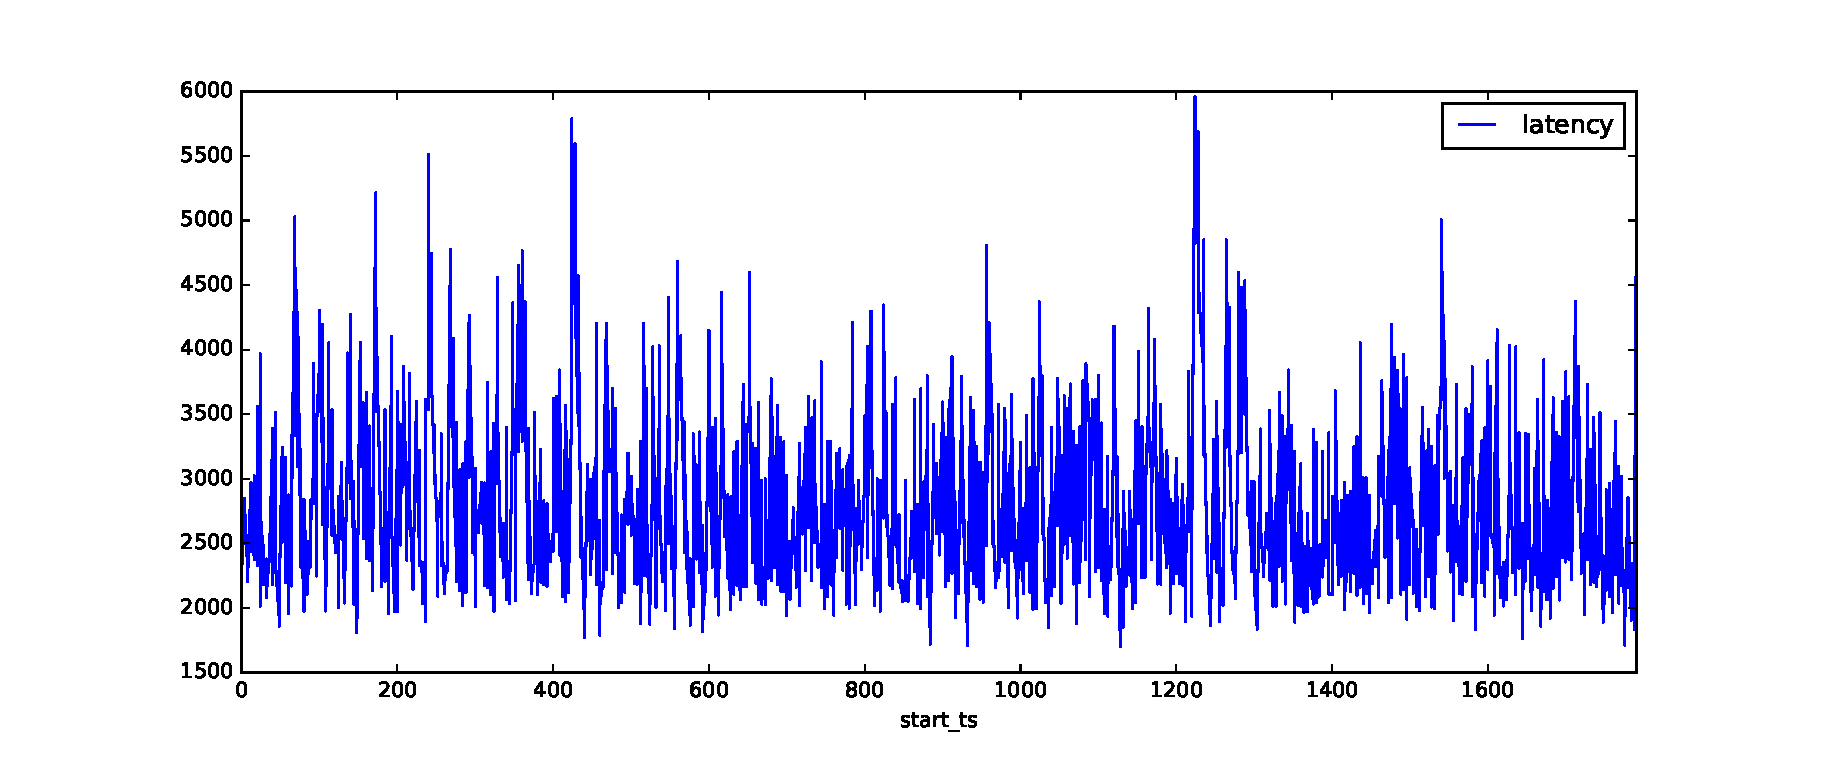
\includegraphics[width=\textwidth]{eps/spark_agg_8node_th_90_ts}

        \caption{Spark, 8-node,  90\%- throughput }
        
    \end{subfigure}



    \begin{subfigure}[b]{0.3\textwidth}
        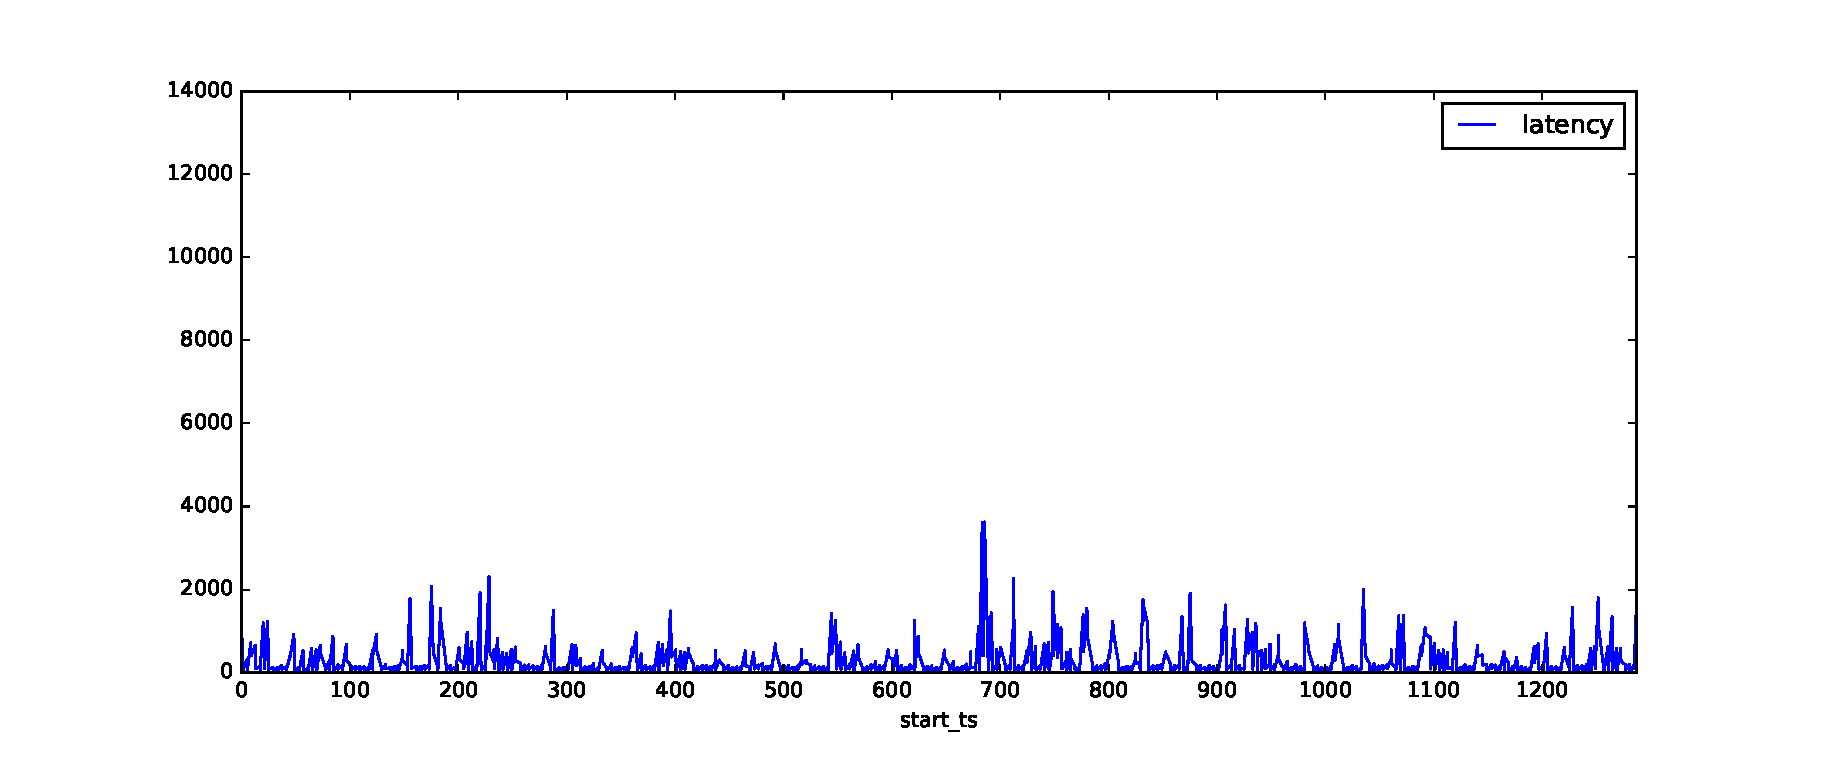
\includegraphics[width=\textwidth]{eps/flink_agg_2node_th_90_ts}

        \caption{Flink, 2-node,  90\%- throughput }
        \label{fig_flink_agg_2node_th_90_ts}
    \end{subfigure}
    ~ 
    \begin{subfigure}[b]{0.3\textwidth}
        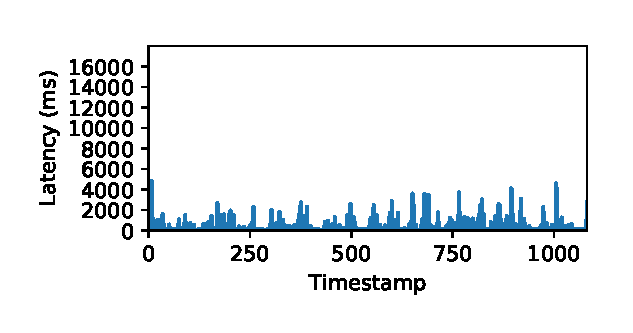
\includegraphics[width=\textwidth]{eps/flink_agg_4node_th_90_ts}

        \caption{Flink, 4-node,  90\%- throughput }
    \end{subfigure}
    ~ 
    \begin{subfigure}[b]{0.3\textwidth}
        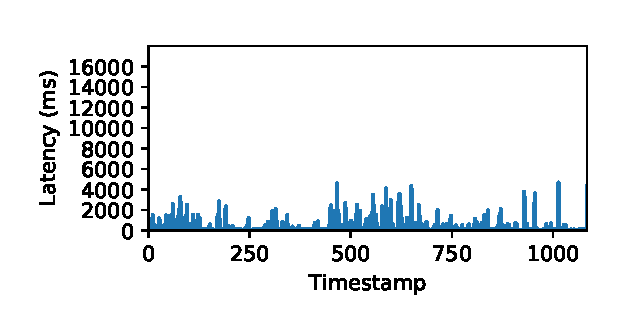
\includegraphics[width=\textwidth]{eps/flink_agg_8node_th_90_ts}

        \caption{Flink, 8-node, 90\% throughput }
        
    \end{subfigure}

        \caption{Windowed aggregation latency distributions in time series}
                \label{fig_ts_agg}
\end{figure*}









Figures \ref{fig_hist_agg} and \ref{fig_ts_agg} show the windowed aggregation latency distributions as  histogram and  time-series,  respectively. 
In all cases we can see that the fluctuations are lowered when decreasing the throughput by 10\%.  While in Storm and in Flink it is hard to detect the lower bounds of latency as they are close to zero, in Spark the upper and lower boundaries are more stable and clearly noticeable. The reason is that a Spark job's characteristics are  highly dependent on the batch size and this determines the clear upper and lower boundaries for the latency. The lower the batch size, the lower the latency and throughput. To have a stable and efficient configuration in Spark, the mini-batch processing time should be less than the batch interval.  We determine the most fluctuating system to be Flink in  2-node setup and Storm in 8-node setup  as shown in Figures \ref{flink_agg_2node_th_max_ts} and \ref{fig_storm_agg_8node_th_max_ts}. Those fluctuations show the behaviour of backpressure. For the same experiment with 90\% of the maximum throughput, we notice that the fluctuations are significantly reduced as shown in  Figures \ref{fig_flink_agg_2node_th_90_ts} and \ref{fig_storm_agg_8node_th_90_ts}.
As we discussed above, 4- and 8-node experiments in Flink are network bound; therefore, these experiments do not fully utilize the Flink nodes and thus have a lower variance in latency. 



Figure \ref{fig_cpu_network_metrics} shows the resource usages of the SUTs. The upper figure shows the CPU load during the experiment. The CPU load is the number of kernel level threads  that are runnable and queued while waiting for CPU resources, averaged over one minute. The next figure shows the network usage of the SUTs.  Because the overall result is similar, we show the of systems' resource utilization graphs  with windowed aggregation case in 4-node cluster.  Because Flink's performance is bounded by network, we can see that CPU utilization is minimal among others. Storm, on the other hand, uses approximately 50\% more CPU clock cycles than Spark. This results in having competitively higher throughout than Spark. One reason behind  Spark's efficient usage of CPU is that Spark automizes most of the work, handles resource usages transparent to user, and does a lot of optimizations internally. For example, Spark handles incremental state management, optimizations with code generation and dynamic memory management efficiently and transparent to user. 



    \begin{table}
        \begin{tabular}{lllll}\toprule
            &\textbf{2-node}  & \textbf{4-node} & \textbf{8-node}\\\midrule
            Spark & 365K & 632K & 947K  \\
            Flink & 851K & 1128K & 1190K \\
        \end{tabular}
        \caption{Sustainable throughput for windowed joins}
                 \label{tab_th_join}
    \end{table} 


\setlength{\tabcolsep}{0.1em} % for the horizontal padding
{\renewcommand{\arraystretch}{1.0}% for the vertical padding
    \begin{table*}
        \resizebox{\textwidth}{!} {\begin{tabular}{lllll}\toprule
            &\textbf{2-node}  & \textbf{4-node} & \textbf{8-node}\\\midrule
            Spark & 7724, 1376, 21600, (11297, 12409, 14718) & 6730, 2139, 23647, (10279, 11788, 15410) & 6263, 1841, 19993, (9465, 10469, 13242) \\
            Spark(90\%) & 7195, 2157, 17981, (10316, 11178, 12702) & 5834, 1861, 13956, (8741, 9525, 10729) & 5788, 1721, 14197, (8678, 9454, 10625)\\
            Flink & 4367, 17, 18230, (7601, 8570, 10554) & 3671, 19, 13872, (6756, 7531, 8664) & 3275, 22, 14934, (6241, 7045, 8436) \\
            Flink(90\%) & 3866, 19, 13027, (6786, 7569, 8759) & 3243, 16, 12702, (6130, 6901, 8011)  & 3240, 16, 14978, (6199, 6995, 8304) \\
        \end{tabular}}
        \caption{Latency statistics, avg, min, max and quantiles (25, 50, 75) in milliseconds for windowed joins.}
                 \label{tab_lat_join}
    \end{table*} 


\begin{figure*}
   \centering

   \begin{subfigure}[b]{0.3\textwidth}
       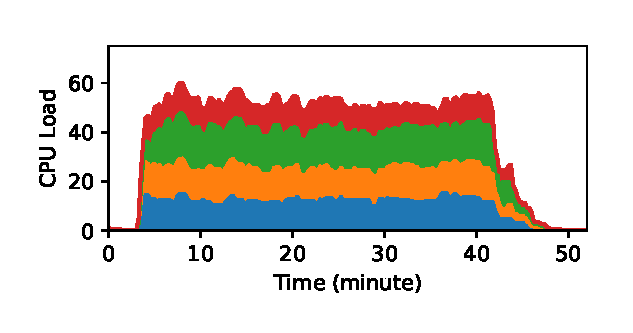
\includegraphics[width=\textwidth]{eps/storm_load_one}
        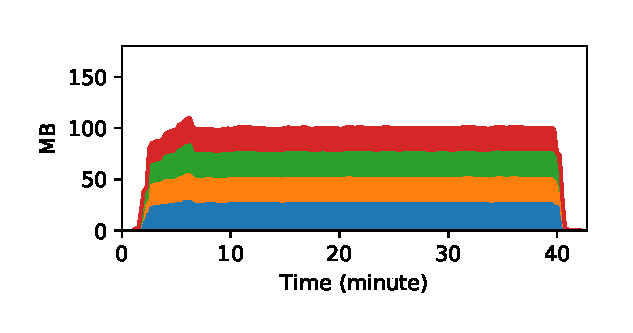
\includegraphics[width=\textwidth]{eps/storm_bytes_in}

       \caption{CPU and network usage of Storm }
   \end{subfigure}
      ~ 
   \begin{subfigure}[b]{0.3\textwidth}
       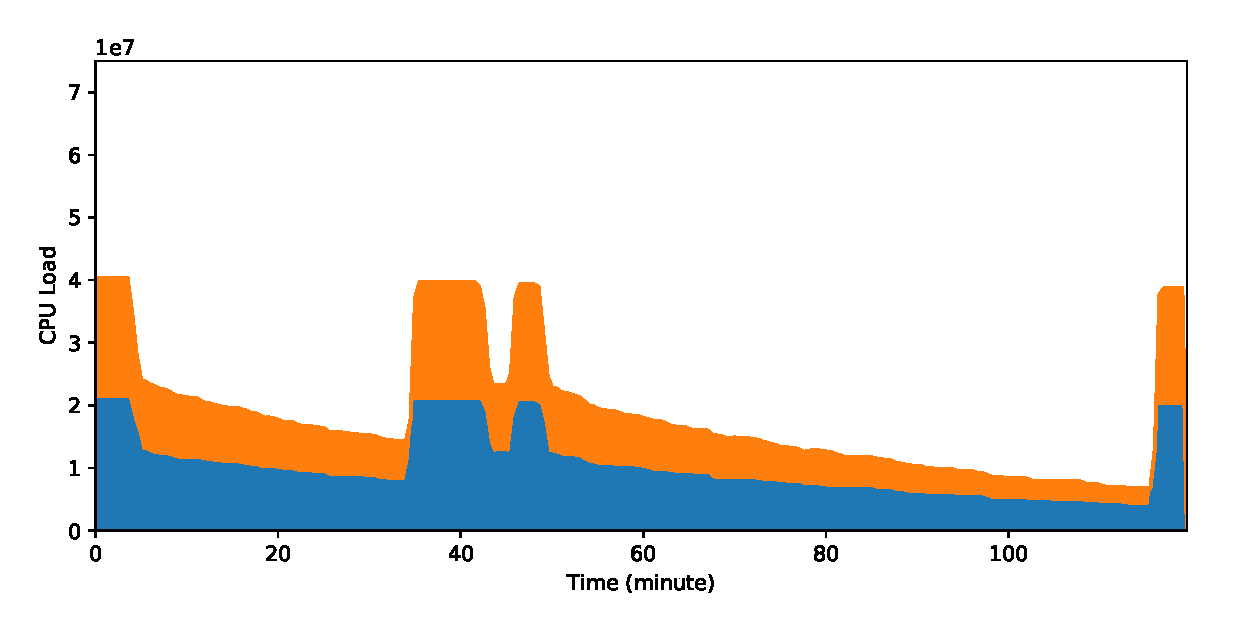
\includegraphics[width=\textwidth]{eps/spark_load_one}
        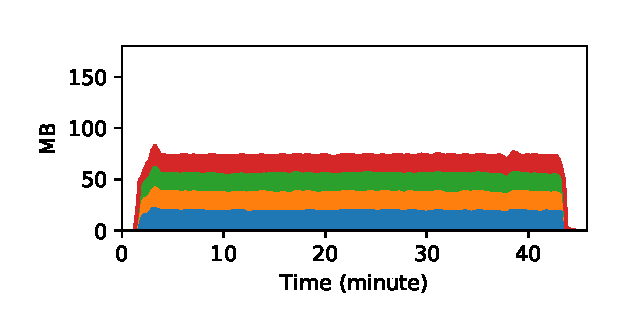
\includegraphics[width=\textwidth]{eps/spark_bytes_in}

       \caption{CPU and network usage of Spark }
   \end{subfigure}
   ~ 
   \begin{subfigure}[b]{0.3\textwidth}
       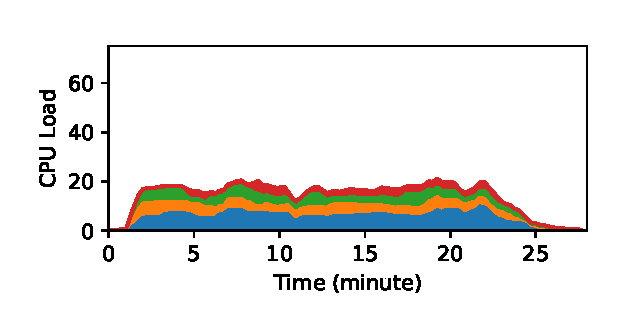
\includegraphics[width=\textwidth]{eps/flink_load_one}
        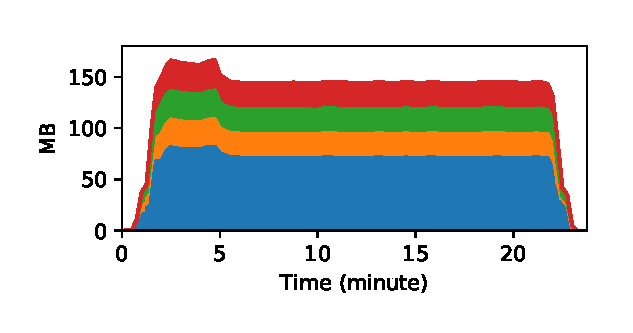
\includegraphics[width=\textwidth]{eps/flink_bytes_in}

       \caption{CPU and network usage of Flink }
   \end{subfigure}

        \caption{CPU and Network usage of systems in a 4-node cluster. Colors indicate nodes in a cluster}
        \label{fig_cpu_network_metrics}
\end{figure*}



\textbf{Event time vs System time latency.}
\textcolor{red}{In this paper we introduce new definition of latency for SDPSs. It is crucial to conduct comparative analysis of event time and system time latency. System time latency is the time interval between tuple's ingestion to SUT and its emission from the sink operator of SUT. Event time latency, on the other hand, is the end-to-end latency between tuple's tuple's event time and its emission time from the sink operator of SUT. Figure \ref{event_vs_system_latency} shows the comparison between the two cases. We conducted this experiments with Query-1, window length = 8 sec, window slide = 4 sec. Event with small cluster size  we can see, there is significant difference between event and system time latency. To be more specific, Storm's $avg$ system time latency is 1234ms (event time is 1407ms), Spark's is 1040ms (even time is 3394ms) and Flink's $avg$ system time latency is 254ms (event time is 563ms). We examined the similar behavior with large cluster size and with join queries as well. }




\begin{figure*}
	\centering
	
	\begin{subfigure}[b]{0.3\textwidth}
		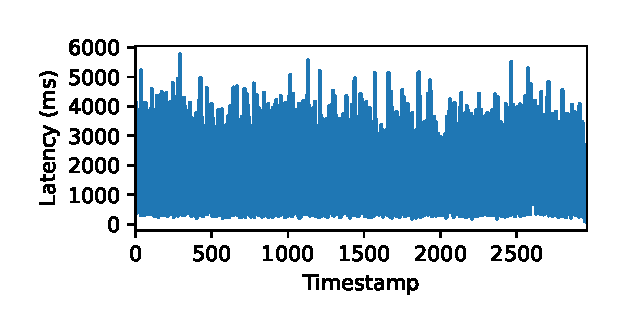
\includegraphics[width=\textwidth]{eps/storm_agg_2node_th_max2_ts}
		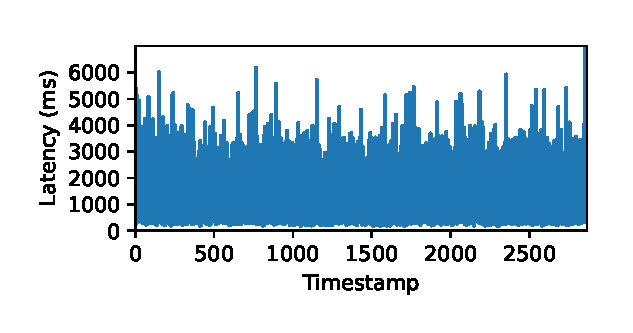
\includegraphics[width=\textwidth]{eps/storm_2node-system_2}
		
		\caption{TODO }
	\end{subfigure}
	~ 
	\begin{subfigure}[b]{0.3\textwidth}
		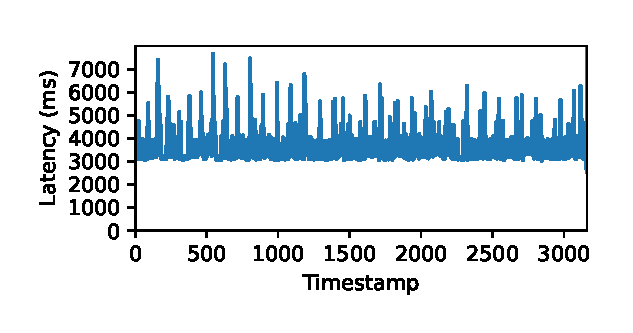
\includegraphics[width=\textwidth]{eps/spark_agg_2node_th_max_2_ts}
		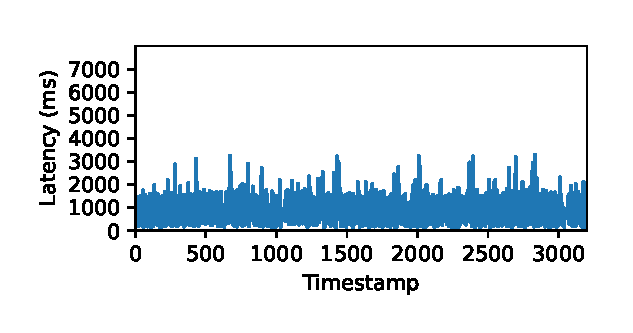
\includegraphics[width=\textwidth]{eps/spark_system_latency_2}
		
		\caption{Event  vs system  time latency in Spark }
	\end{subfigure}
	~ 
	\begin{subfigure}[b]{0.3\textwidth}
		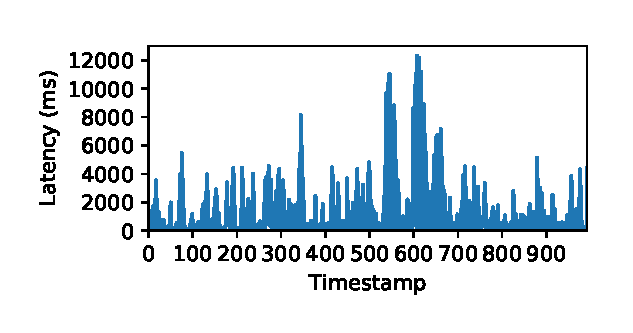
\includegraphics[width=\textwidth]{eps/flink_agg_2node_th_max_2_ts}
		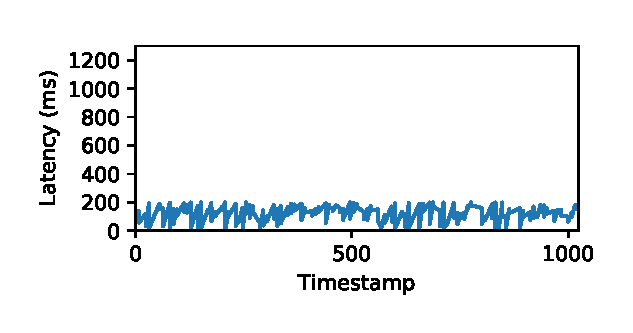
\includegraphics[width=\textwidth]{eps/flink_system_latency_1}
		
		\caption{Event vs system time latency in Flink }
	\end{subfigure}
	
	\caption{\textcolor{red}{Comparison between event and system time latency among systems}}
	\label{event_vs_system_latency}
\end{figure*}











\textbf{More throughput  than a system can sustain.}
\textcolor{red}{Providing maximum sustainable throughput to SDPSs is essential as otherwise the performance of the systems can degrade. We experienced on average 5-10 \% performance decrease on 20\% more throughput than the system can sustain. We did experiments with Query-1 and Query-2 with window length between 5-10 second, and window slide between 1-5 seconds. We experienced that as the window size gets large and window slide and buffer size gets smaller, Storm's probability to drop the sockets increases. In general the decrease in overall throughput is dominated by the time interval where the system is unstable, meaning the system cannot fire the backpressure effectively. For example, we executed Query-1 with window length = 8 seconds and window slide = 4 seconds on 2 nodes. The overall throughput of the Storm, Spark and Flink decreased by 6\%, 5\%, 3\%  respectively. With the same parameters on Query-2, we examined approximately 1.5 times more performance decrease with 20\% more throughput. Moreover, if the data is skewed the performance loss can be in orders of magnitude (in Spark, Figure \ref{more_th}) or even system failure (in Flink).   }


\begin{figure}
	\centering
	
	\begin{subfigure}[b]{0.45\textwidth}
		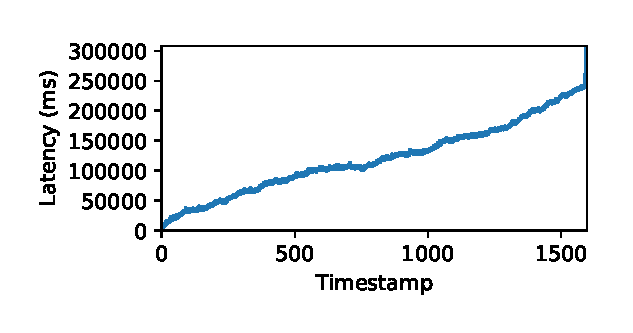
\includegraphics[width=\textwidth]{eps/storm_system_more_th_1}

		
		\caption{System time latency }
	\end{subfigure}
	~ 
	\begin{subfigure}[b]{0.45\textwidth}
		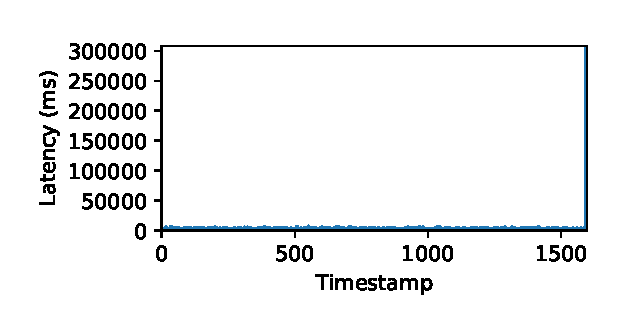
\includegraphics[width=\textwidth]{eps/storm_system_more_th_2}
		
		\caption{Event time latency }
	\end{subfigure}

	
	\caption{Event vs system latency with more workload than Spark can sustain}
	\label{more_th}
\end{figure}



\textbf{Impact of window size to systems' performance.}
\textcolor{red}{The window size and window slide has significant impact on system's performance with windowed operations. Here we talk about partitioned windowed operations as Spark is single winner in global windows in scale. One interesting fact we inspected is that with the increasing window size Spark's throughput decreases significantly given the same batch size. For example, with window length and slide 60 seconds, Spark's throughput decreases by 2 times and avg latency increases by 10 times given the batch size 4 seconds. However, with higher batch sizes, Spark can handle much higher workloads and big windows. Storm on the other hand, can handle the big window sized operations if the user has advanced data structures that can spill to disk when needed. Otherwise, we encountered memory exceptions. Flink (as well as Spark) has built-in data structures that can spill to disk when needed. However, this do not apply for the operations inside the UDFs, as Flink treats UDFs as blackbox. }


\begin{figure}
	\centering
	\begin{subfigure}[b]{0.5\textwidth}
		\includegraphics[width=\textwidth]{eps/spark_skewed_join_1}
		
		\caption{Event time latency (79175.5)}
		\label{fig_spark_join_2node_th_max_ts}
	\end{subfigure}%
	\begin{subfigure}[b]{0.5\textwidth}
		\includegraphics[width=\textwidth]{eps/spark_skewed_join_2}
		
		\caption{System latency (77181.6) }
		\label{fig_spark_join_4node_th_max_ts}
	\end{subfigure}%
	\caption{Event vs system latency with skewed data}
	\label{skew}
\end{figure}

\textbf{Impact of data skew to systems' performance.}
\textcolor{red}{Data skew is another factor affecting the system performance. Especially in industrial scenarios one should not expect purely equal data distribution. We tested the systems with extreme skew, which is with single key. Here, we treat Flink's global windowed performance equivalently for skewed data with one key. The reason is that, Flink internally uses static dummy key to partition global windows. The similar approach is used in Storm as well. Spark on the other hand, can handle skewed data efficiently. We experienced Spark outperforming both engines with Query-1 (8sec, 4sec) in a cluster with 4 nodes or more. For skewed joins on the other hand, both Spark and Flink stugle to handle. Flink often got stuck and stayed unresponsive in this case. Spark on the other hand, performed with very high latencies. We decreased the join operator's selectivity to make sure that data transfer is not a bottleneck. The main reason is that the memory is consumed quite fast and backpressure mechanism lacks to perform efficiently. As can be seen from Figure \ref{skew}, although very high latency the system, Spark in this case, ingests the input continuously. }



\begin{figure*}
	\centering
	
	\begin{subfigure}[b]{0.3\textwidth}
		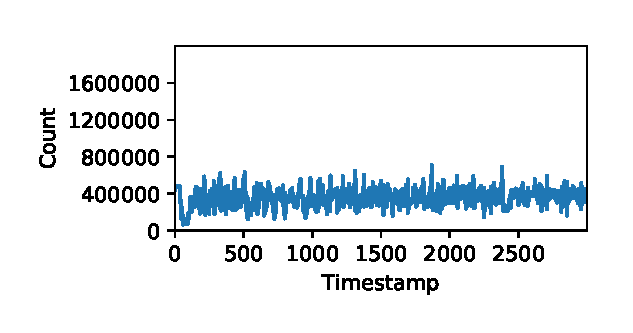
\includegraphics[width=\textwidth]{eps/storm_pull_pg}
		
		
		\caption{Storm }
	\end{subfigure}
	~ 
	\begin{subfigure}[b]{0.3\textwidth}
		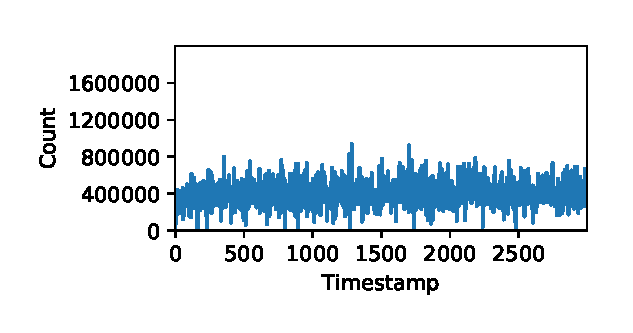
\includegraphics[width=\textwidth]{eps/spark_pull_pg}
		
		
		\caption{ Spark }
	\end{subfigure}
	~ 
	\begin{subfigure}[b]{0.3\textwidth}
		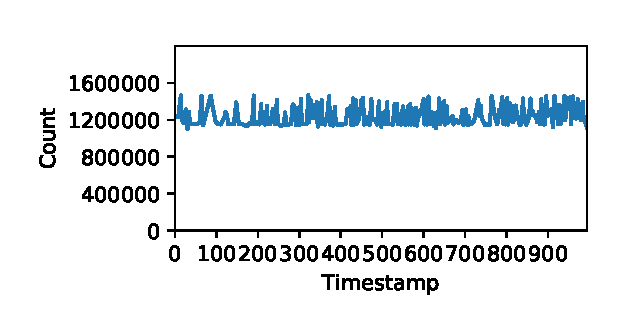
\includegraphics[width=\textwidth]{eps/flink_pull_pg}
		
		
		\caption{ Flink }
	\end{subfigure}
	
	\caption{\textcolor{red}{Data pull graphs of systems}}
	\label{pull_graph}
\end{figure*}




\textbf{Data pulling from data source.}
\textcolor{red}{While analyzing the systems' performance it is essential to inspect their data pull graphs from data sources. We retrieved this metrics from driver side to ensure that we are not affecting the system performance. Figure \ref{pull_graph} shows the corresponding behavior of systems with maximum sustainable throughout on Query-1 (8sec, 4sec). However we examined the similar behavior in other window settings and windowed operations as long as the workload is maximum sustainable.  As we can see, Spark and Storm have fluctuating data pull rates. Despite having high data pull rate, Flink have less fluctuations. Once we lower the workload both Flink and Spark gets to monotonic data pull rate; however, Storm still exibits significant fluctuations. }



\begin{figure*}
	\centering
	
	\begin{subfigure}[b]{0.3\textwidth}
		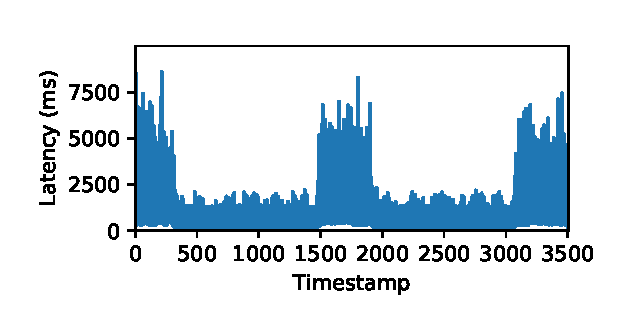
\includegraphics[width=\textwidth]{eps/storm_peak_agg_1}
		
		
		\caption{Storm aggregation }
	\end{subfigure}
	~ 
	\begin{subfigure}[b]{0.3\textwidth}
		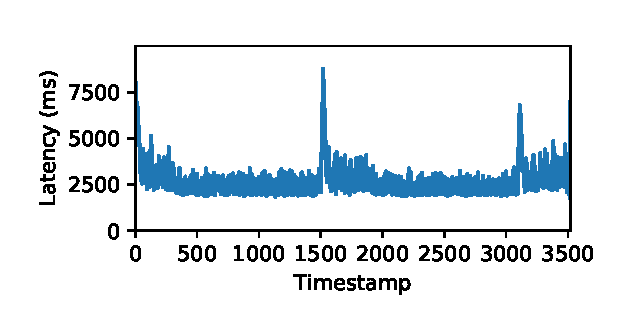
\includegraphics[width=\textwidth]{eps/spark_peak_agg_1}
		
		
		\caption{ Spark aggregation }
	\end{subfigure}
	~ 
	\begin{subfigure}[b]{0.3\textwidth}
		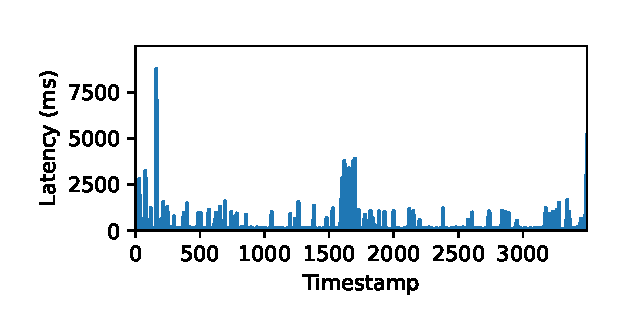
\includegraphics[width=\textwidth]{eps/flink_peak_agg_1}
		
		
		\caption{ Flink aggregation}
	\end{subfigure}
	~ 
	\begin{subfigure}[b]{0.3\textwidth}
		
		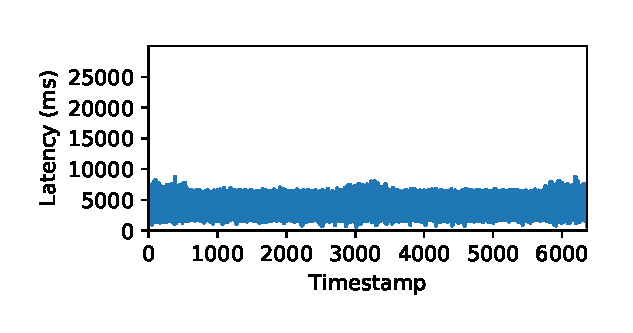
\includegraphics[width=\textwidth]{eps/spark_peak_join_2}

		\caption{Spark system time latency }
		\label{peaks_system_time}
	\end{subfigure}
	~ 
	\begin{subfigure}[b]{0.3\textwidth}
		
		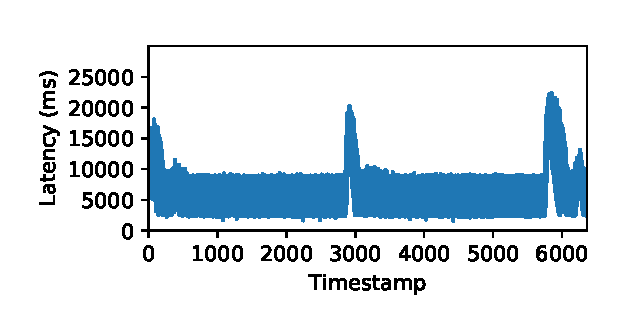
\includegraphics[width=\textwidth]{eps/spark_peak_join_1}

		\caption{ Spark join}
		\label{peaks_spark_join}
	\end{subfigure}
	~ 
	\begin{subfigure}[b]{0.3\textwidth}
		
		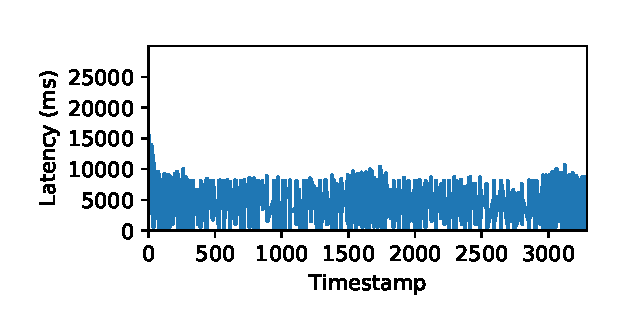
\includegraphics[width=\textwidth]{eps/flink_peak_join_1}
		
		\caption{ Flink join }
	\end{subfigure}
	\caption{\textcolor{red}{Peaks}}
	\label{peaks}
\end{figure*}


\textbf{Peaks.}
\textcolor{red}{Especially in industrial scenario, peaks are inevitable. We simulated the peaks for all systems both for Query-1(8 sec, 4 sec) and Query-2 (8sec, 4sec). We start the benchmark with 840K per second workload then decrease it to 280K and increase again after a while.   As can be seen from Figure \ref{peaks}, Storm is the most susceptible system for peaks. Spark and Flink have comparative behavour with partitioned windowed aggregations case. However, for partitioned windowed join case, Flink can handle peaks better. To emphasize the event and system time latency again, we show the system time latency of Figure \ref{peaks_spark_join} in Figure \ref{peaks_system_time}.  }

\textbf{Another scenarios}
\textcolor{red}{To test the systems' behavour deeply, we conducted more complex scenario with Query-3. The main purpose is to inspect engines' query optimization with non-trivial queries. Examining the logical and physical query graph, we inspect that Flink and Spark perform query optimization techniques to increase the performance of system. Therefore, the performance of systems stay approximately with the same proportion, with a more complex query. The same can be said about lower workloads. We tested systems with lower workloads than they can sustain. One interesting behaviour was that  Flink's avg latency increase with the smaller workloads. So we had to tune the buffer size for each workload to lower the latency; however, in real industrial scenario this is not the case. In Spark however, the avg latency improved with decreasing workloads. However, it can be further improved with smaller batch size. For this, again we have to stop the job and tune the system for each workload, which is unrealistic in real industrial scenarios. 
Number of keys}























\textbf{Windowed Joins}
In the second use-case, we use partitioned windowed joins in Spark and Flink.
  Storm provides a windowing capability but there is no built-in windowed join operator. Initially, we tried Storm's Trident abstrac\-tion, which has built-in windowed join features. However, Trident computed incorrect results as we increased the batch size. Moreover, there is a lack of support for Trident in the Storm community. As an alternative, we implemented a simple version of a windowed join in Storm. However, comparing it with Spark and Flink, which have advanced memory and state management features, leads to unfair comparisons. We implemented a na\"ive join in Storm and examined the maximum sustainable throughput to be 140K events per second and measured an average latency of 2349 milliseconds  on a 2-node cluster. However, we faced memory issues and topology stalls on larger clusters. 
%Moreover, this  would be highly implementation dependent. 
As a result, we focus on Flink and Spark in our windowed join benchmarks.

Throughout the experiments, we found important points that need to be taken into consideration while performing windowed joins over streams. First, depending on the selectivity of the input streams to the join operator, vast amount of results can be produced which can limit the speed of the engine to the disk I/O. We are assuming that the result sink is a file system. Second, the vast amount of results of a join operator can cause the network to be a bottleneck. This can happen if we output the results to shared file system. If the result size is large, then the network becomes a bottleneck. To address this issue, we decreased the selectivity of the input streams.  In general, the experimental results for windowed joins are similar to the experiments with windowed aggregations. 

Table \ref{tab_th_join} shows the maximum throughput that the systems under test can sustain.  Flink's throughput for 8-node configuration is bounded by network bandwidth. This is 1256K in windowed aggregations. The reason for the difference is that there is more network traffic as the result size is larger in windowed joins than in windowed aggregations. Tab\-le \ref{tab_lat_join} shows the latency statistics for windowed joins. We can see that  
in all cases Flink outperforms Spark in all parameters. To ensure the stability of the system, the run time of each mini-batch should be less than batch size in Spark. Otherwise, the queued mini-batch jobs will increase over time and the system will not be able to sustain the throughput. However, we see from Table \ref{tab_th_join} that the latency values are higher than mini-batch duration (4 sec). The reason is that we are measuring the event time latency.Therefore, if the latency is higher than mini-batch duration, then the tuples wait in the DQS.

























































\begin{figure*}
    \centering
   \begin{subfigure}[b]{0.3\textwidth}
       \includegraphics[width=\textwidth]{eps/spark_join_2node_th_max_ts}

       \caption{Spark, 2-node, max  throughput}
       \label{fig_spark_join_2node_th_max_ts}
   \end{subfigure}%
   \begin{subfigure}[b]{0.3\textwidth}
       \includegraphics[width=\textwidth]{eps/spark_join_4node_th_max_ts}

       \caption{Spark, 4-node, max  throughput }
              \label{fig_spark_join_4node_th_max_ts}
   \end{subfigure}%
   \begin{subfigure}[b]{0.3\textwidth}
       \includegraphics[width=\textwidth]{eps/spark_join_8node_th_max_ts}

       \caption{Spark, 8-node, max  throughput }
              \label{fig_spark_join_8node_th_max_ts}
   \end{subfigure}




   \begin{subfigure}[b]{0.3\textwidth}
       \includegraphics[width=\textwidth]{eps/flink_join_2node_th_max_ts}

       \caption{Flink, 2-node, max  throughput}
   \end{subfigure}%
   \begin{subfigure}[b]{0.3\textwidth}
       \includegraphics[width=\textwidth]{eps/flink_join_4node_th_max_ts}

       \caption{Flink, 4-node, max  throughput }
   \end{subfigure}%
   \begin{subfigure}[b]{0.3\textwidth}
       \includegraphics[width=\textwidth]{eps/flink_join_8node_th_max_ts}

       \caption{Flink, 8-node, max  throughput }
   \end{subfigure}
   
   
   
   
      \begin{subfigure}[b]{0.3\textwidth}
       \includegraphics[width=\textwidth]{eps/spark_join_2node_th_90_ts}

       \caption{Spark, 2-node,  90\%-throughput}
   \end{subfigure}%
   \begin{subfigure}[b]{0.3\textwidth}
       \includegraphics[width=\textwidth]{eps/spark_join_4node_th_90_ts}

       \caption{Spark, 4-node,  90\%-throughput }
   \end{subfigure}%
   \begin{subfigure}[b]{0.3\textwidth}
       \includegraphics[width=\textwidth]{eps/spark_join_8node_th_90_ts}

       \caption{Spark, 8-node,  90\%-throughput }
   \end{subfigure}




   \begin{subfigure}[b]{0.3\textwidth}
       \includegraphics[width=\textwidth]{eps/flink_join_2node_th_90_ts}

       \caption{Flink, 2-node,  90\%-throughput}
   \end{subfigure}
   ~ 
   \begin{subfigure}[b]{0.3\textwidth}
       \includegraphics[width=\textwidth]{eps/flink_join_4node_th_90_ts}

       \caption{Flink, 4-node,  90\%-throughput }
   \end{subfigure}
   ~ 
   \begin{subfigure}[b]{0.3\textwidth}
       \includegraphics[width=\textwidth]{eps/flink_join_8node_th_90_ts}

       \caption{Flink, 8-node,  90\%-throughput }
   \end{subfigure}

        \caption{Windowed join latency distributions in time series}
                \label{fig_ts_join}
\end{figure*}













Figures  \ref{fig_hist_join} and \ref{fig_ts_join} show the latency for the windowed joins case as  histogram and time-series .  In contrast to windowed aggregations, we see the substantial fluctuations in Spark in Figures \ref{fig_spark_join_2node_th_max_ts}, \ref{fig_spark_join_4node_th_max_ts} and \ref{fig_spark_join_8node_th_max_ts}.
Also we can see a significant latency increase in Flink when compared to windowed aggregation experiments. The reason is that windowed joins are   more expensive than windowed aggregations. However, the spikes are significantly reduced with 90\% workload.  


\subsection{Discussion}

%Given the benchmarking system and the output, we derive  conclusions out of experimental results. In general there is no single winner and each system is good for specific use-case as all three SUTs have large communities and considerable amount of support in industry. However, it is important to notice the key points derived out of this experiments. 

% \todo[inline]{Please reduce the generic sentences, this is obvious=>fixed}
 
Throughout the experiments, we notice that Storm has a comparable performance  to Spark. Storm could provide more high level abstractions  with transparent on/of-heap memory management in the engine. We can see from resource utilization graphs that the usage of low level APIs results to high CPU and network usage in system.  Although Trident is a high level abstraction on top of Storm, its efficiency is much lower than Storm and with large batch sizes, it produces wrong results. Moreover, Storm's backpressure mechanism needs further enhancements as it can stall the topology with high throughputs.

Although Spark performs worse than Storm in terms of throughput, its high level APIs and advanced and the dynamic memory management is better than Storm and competitive with Flink. One downside of Spark is that it schedules one job at a time. So there is only one active job at a time.  Although there is an experimental feature to start multiple mini-batch jobs at a time, this can lead to unexpected sharing of resources. Moreover, Spark's backpressure mechanism was significantly improved  in recent releases but there is still need for further improvement. 

Flink performs best in throughput and in $avg$ latency. However, its $max$ latency is worse in comparison to other systems. Flink could add a dynamic buffer management feature to change the size of buffers at runtime to reduce the latency. We noticed the performance of Flink's backpressure to be the best because of its robustness and its low overhead.


There is no single winner according to the experimental results. Storm's and Spark's throughputs in windowed aggregations are comparable but in terms of $avg$ latency Storm is better. So if a user needs to use lower level APIs to implement custom business logic, then Storm is the best engine for windowed aggregation. However, Spark reduces latency when scaling out. So, when working with very large clusters Spark can outperform Storm. Flink on the other hand, provides the highest throughput and the lowest  $avg$ latency with its transparent and high level APIs. However, its  high $max$ latency is a limitation when compared to other systems.  







%\todo[inline]{This is still a bit unstructured, maybe you can get the overall comparison in order, e.g., per system and then total}































%    \begin{table}
        \begin{tabular}{lllll}\toprule
            &\textbf{2 Node}  & \textbf{4 Node} & \textbf{8 Node}\\\midrule
            Storm & 408K & 696K & XXX  \\
            Spark & 379K & 642K & 912K  \\
            Flink & 1230K & *1260K & *1260K \\
            \\\bottomrule
        \end{tabular}
        \caption{Sustainable throughput for windowed aggregations}\label{Tab1}
    \end{table} 



    \begin{table}
        \begin{tabular}{lllll}\toprule
            &\textbf{2 Node}  & \textbf{4 Node} & \textbf{8 Node}\\\midrule
            Storm & 1424ms & 2043ms & XXX \\
            Storm(90\%) & 1109ms & 1669ms & XXX \\
            Spark & 3759ms & 4138ms & 3152ms\\
            Spark(90\%) & 3418ms & 2846ms & 2798ms\\
            Flink & 576ms & 259ms & 243ms \\
            Flink(90\%) & 299ms & -  & - \\
            \\\bottomrule
        \end{tabular}
        \caption{Average Latency for windowed aggregations}\label{Tab1}
    \end{table} 


    \begin{table}
        \begin{tabular}{lllll}\toprule
            &\textbf{2 Node}  & \textbf{4 Node} & \textbf{8 Node}\\\midrule
            Storm & xxx & xxx & XXX  \\
            Spark & 365K & 632K & 947K  \\
            Flink & 851K & 1128K & *1260K \\
            \\\bottomrule
        \end{tabular}
        \caption{Sustainable throughput for windowed joins}\label{Tab1}
    \end{table} 



    \begin{table}
        \begin{tabular}{lllll}\toprule
            &\textbf{2 Node}  & \textbf{4 Node} & \textbf{8 Node}\\\midrule
            Storm & 1424ms & 2043ms & XXX \\
            Storm(90\%) & 1109ms & 1669ms & XXX \\
            Spark & 8417ms & 7823ms & 7590ms\\
            Spark(90\%) & 7538ms & 5825ms & 6015ms\\
            Flink & 4825ms & 4255ms & *3748ms \\
            Flink(90\%) & 3872ms & 3285ms  & - \\
            \\\bottomrule
        \end{tabular}
        \caption{Average Latency for windowed joins}\label{Tab1}
    \end{table} 

%\begin{figure*}
    \centering
    \begin{subfigure}[b]{0.3\textwidth}
        \includegraphics[width=\textwidth]{eps/storm_agg_2node_th_max_hist}
         \includegraphics[width=\textwidth]{eps/storm_agg_2node_th_max_ts}

        \caption{2 Node latency with max throughput}
    \end{subfigure}
    ~ 
    \begin{subfigure}[b]{0.3\textwidth}
        \includegraphics[width=\textwidth]{eps/storm_agg_4node_th_max_hist}
         \includegraphics[width=\textwidth]{eps/storm_agg_4node_th_max_ts}

        \caption{4 Node latency with max throughput }
    \end{subfigure}
    ~ 
    \begin{subfigure}[b]{0.3\textwidth}
        \includegraphics[width=\textwidth]{eps/storm_agg_8node_th_max_hist}
         \includegraphics[width=\textwidth]{eps/storm_agg_8node_th_max_ts}

        \caption{8 Node latency with max throughput }
    \end{subfigure}




    \begin{subfigure}[b]{0.3\textwidth}
        \includegraphics[width=\textwidth]{eps/storm_agg_2node_th_90_hist}
         \includegraphics[width=\textwidth]{eps/storm_agg_2node_th_90_ts}

        \caption{2 Node latency with 90\% throughput }
    \end{subfigure}
    ~ 
    \begin{subfigure}[b]{0.3\textwidth}
        \includegraphics[width=\textwidth]{eps/storm_agg_4node_th_90_hist}
         \includegraphics[width=\textwidth]{eps/storm_agg_4node_th_90_ts}

        \caption{4 Node latency with 90\% throughput }
    \end{subfigure}
    ~ 



        \caption{Latency of windowed aggregations for Storm}
\end{figure*}
%\begin{figure*}
    \centering
    \begin{subfigure}[b]{0.3\textwidth}
        \includegraphics[width=\textwidth]{eps/spark_agg_2node_th_max_hist}
         \includegraphics[width=\textwidth]{eps/spark_agg_2node_th_max_ts}

        \caption{2 Node latency with max throughput}
    \end{subfigure}
    ~ 
    \begin{subfigure}[b]{0.3\textwidth}
        \includegraphics[width=\textwidth]{eps/spark_agg_4node_th_max_hist}
         \includegraphics[width=\textwidth]{eps/spark_agg_4node_th_max_ts}

        \caption{4 Node latency with max throughput }
    \end{subfigure}
    ~ 
    \begin{subfigure}[b]{0.3\textwidth}
        \includegraphics[width=\textwidth]{eps/spark_agg_8node_th_max_hist}
         \includegraphics[width=\textwidth]{eps/spark_agg_8node_th_max_ts}

        \caption{8 Node latency with max throughput }
    \end{subfigure}




    \begin{subfigure}[b]{0.3\textwidth}
        \includegraphics[width=\textwidth]{eps/spark_agg_2node_th_90_hist}
         \includegraphics[width=\textwidth]{eps/spark_agg_2node_th_90_ts}

        \caption{2 Node latency with 90\% throughput }
    \end{subfigure}
    ~ 
    \begin{subfigure}[b]{0.3\textwidth}
        \includegraphics[width=\textwidth]{eps/spark_agg_4node_th_90_hist}
         \includegraphics[width=\textwidth]{eps/spark_agg_4node_th_90_ts}

        \caption{4 Node latency with 90\% throughput }
    \end{subfigure}
    ~ 
    \begin{subfigure}[b]{0.3\textwidth}
        \includegraphics[width=\textwidth]{eps/spark_agg_8node_th_90_hist}
         \includegraphics[width=\textwidth]{eps/spark_agg_8node_th_90_ts}

        \caption{8 Node latency with 90\% throughput }
    \end{subfigure}



        \caption{Latency of windowed aggregations for Spark}
\end{figure*}
%\begin{figure*}
    \centering
    \begin{subfigure}[b]{0.3\textwidth}
        \includegraphics[width=\textwidth]{eps/flink_agg_2node_th_max_hist}
         \includegraphics[width=\textwidth]{eps/flink_agg_2node_th_max_ts}

        \caption{2 Node latency with maximum throughput}
    \end{subfigure}
    ~ 
    \begin{subfigure}[b]{0.3\textwidth}
        \includegraphics[width=\textwidth]{eps/flink_agg_4node_th_max_hist}
         \includegraphics[width=\textwidth]{eps/flink_agg_4node_th_max_ts}

        \caption{4 Node latency with network bounded throughput }
    \end{subfigure}
   ~
    \begin{subfigure}[b]{0.3\textwidth}
        \includegraphics[width=\textwidth]{eps/flink_agg_8node_th_max_hist}
         \includegraphics[width=\textwidth]{eps/flink_agg_8node_th_max_ts}

        \caption{8 Node latency with network bounded throughput }
    \end{subfigure}
    ~ 
    \begin{subfigure}[b]{0.3\textwidth}
        \includegraphics[width=\textwidth]{eps/flink_agg_2node_th_90_hist}
         \includegraphics[width=\textwidth]{eps/flink_agg_2node_th_90_ts}

        \caption{2 Node latency with 90\% throughput }
    \end{subfigure}
    ~ 
    \begin{subfigure}[b]{0.3\textwidth}
        \includegraphics[width=\textwidth]{eps/flink_agg_4node_th_90_hist}
         \includegraphics[width=\textwidth]{eps/flink_agg_4node_th_90_ts}

        \caption{2 Node latency with 90\% throughput }
    \end{subfigure}
    ~ 
    \begin{subfigure}[b]{0.3\textwidth}
        \includegraphics[width=\textwidth]{eps/flink_agg_8node_th_90_hist}
         \includegraphics[width=\textwidth]{eps/flink_agg_8node_th_90_ts}

        \caption{2 Node latency with 90\% throughput }
    \end{subfigure}




        \caption{Latency of windowed aggregations for Flink}
\end{figure*}
%\begin{figure*}
    \centering
    \begin{subfigure}[b]{0.3\textwidth}
        \includegraphics[width=\textwidth]{eps/spark_join_2node_th_max_hist}
         \includegraphics[width=\textwidth]{eps/spark_join_2node_th_max_ts}

        \caption{2 Node latency with max throughput}
    \end{subfigure}
    ~ 
    \begin{subfigure}[b]{0.3\textwidth}
        \includegraphics[width=\textwidth]{eps/spark_join_4node_th_max_hist}
         \includegraphics[width=\textwidth]{eps/spark_join_4node_th_max_ts}

        \caption{4 Node latency with max throughput }
    \end{subfigure}
    ~ 
    \begin{subfigure}[b]{0.3\textwidth}
        \includegraphics[width=\textwidth]{eps/spark_join_8node_th_max_hist}
         \includegraphics[width=\textwidth]{eps/spark_join_8node_th_max_ts}

        \caption{8 Node latency with max throughput }
    \end{subfigure}




    \begin{subfigure}[b]{0.3\textwidth}
        \includegraphics[width=\textwidth]{eps/spark_join_2node_th_90_hist}
         \includegraphics[width=\textwidth]{eps/spark_join_2node_th_90_ts}

        \caption{2 Node latency with 90\% throughput }
    \end{subfigure}
    ~ 
    \begin{subfigure}[b]{0.3\textwidth}
        \includegraphics[width=\textwidth]{eps/spark_join_4node_th_90_hist}
         \includegraphics[width=\textwidth]{eps/spark_join_4node_th_90_ts}

        \caption{4 Node latency with 90\% throughput }
    \end{subfigure}
    ~ 
    \begin{subfigure}[b]{0.3\textwidth}
        \includegraphics[width=\textwidth]{eps/spark_join_8node_th_90_hist}
         \includegraphics[width=\textwidth]{eps/spark_join_8node_th_90_ts}

        \caption{8 Node latency with 90\% throughput }
    \end{subfigure}



        \caption{Latency of windowed join for Spark}
\end{figure*}
%\begin{figure*}
   \centering
   \begin{subfigure}[b]{0.3\textwidth}
       \includegraphics[width=\textwidth]{eps/flink_join_2node_th_max_hist}
        \includegraphics[width=\textwidth]{eps/flink_join_2node_th_max_ts}

       \caption{2 Node latency with max throughput}
   \end{subfigure}
   ~ 
   \begin{subfigure}[b]{0.3\textwidth}
       \includegraphics[width=\textwidth]{eps/flink_join_4node_th_max_hist}
        \includegraphics[width=\textwidth]{eps/flink_join_4node_th_max_ts}

       \caption{4 Node latency with max throughput }
   \end{subfigure}
   ~ 
   \begin{subfigure}[b]{0.3\textwidth}
       \includegraphics[width=\textwidth]{eps/flink_join_8node_th_max_hist}
        \includegraphics[width=\textwidth]{eps/flink_join_8node_th_max_ts}

       \caption{8 Node latency with max throughput }
   \end{subfigure}




   \begin{subfigure}[b]{0.3\textwidth}
       \includegraphics[width=\textwidth]{eps/flink_join_2node_th_90_hist}
        \includegraphics[width=\textwidth]{eps/flink_join_2node_th_90_ts}

       \caption{2 Node latency with 90\% throughput }
   \end{subfigure}
   ~ 
   \begin{subfigure}[b]{0.3\textwidth}
       \includegraphics[width=\textwidth]{eps/flink_join_4node_th_90_hist}
        \includegraphics[width=\textwidth]{eps/flink_join_4node_th_90_ts}

       \caption{4 Node latency with 90\% throughput }
   \end{subfigure}
   ~ 
   \begin{subfigure}[b]{0.3\textwidth}
       \includegraphics[width=\textwidth]{eps/flink_join_8node_th_90_hist}
        \includegraphics[width=\textwidth]{eps/flink_join_8node_th_90_ts}

       \caption{4 Node latency with 90\% throughput }
   \end{subfigure}



        \caption{Latency of windowed join for Flink}
\end{figure*}











